\documentclass[letterpaper]{article} % DO NOT CHANGE THIS
% AAAI-27 Author Kit (official, https://aaai.org/authorkit27/, AuthorKit27.zip, aaai2027.sty dated 2026-10-21).
% Anonymous-submission mode; author information is a placeholder pending the user's decision.
\usepackage[submission]{aaai2027}  % DO NOT CHANGE THIS
\usepackage[hyphens]{url}  % DO NOT CHANGE THIS
\usepackage{graphicx} % DO NOT CHANGE THIS
\urlstyle{rm} % DO NOT CHANGE THIS
\def\UrlFont{\rm}  % DO NOT CHANGE THIS
\usepackage{natbib}  % DO NOT CHANGE THIS AND DO NOT ADD ANY OPTIONS TO IT
\usepackage{caption} % DO NOT CHANGE THIS AND DO NOT ADD ANY OPTIONS TO IT
\frenchspacing  % DO NOT CHANGE THIS
\usepackage{algorithm}
\usepackage{algorithmic}
\usepackage{booktabs}
\usepackage{array}
\usepackage{amsmath}
\usepackage{placeins} % \FloatBarrier keeps appendix floats in their sections
\pdfinfo{
/TemplateVersion (2027.1)
}
\setcounter{secnumdepth}{2} % Section numbers enabled (permitted by the template: 0, 1 or 2).

\title{
%BrickForma: Text-Driven Generation via Voxel-to-Brick Data Construction and Geometric Reconstruction
%xiao
BrickForma: Crystallizing LLM Geometric Knowledge \\into Small Models for Text-to-Brick Assembly
%xiao
}
% Title confirmed by the author: BrickForma.
\author{
    % TODO 待用户确认: author names and affiliations are placeholders until the user provides them.
    Author Name(s) to Be Added\textsuperscript{\rm 1}
}
\affiliations{
    \textsuperscript{\rm 1}Affiliation(s) to Be Added\\
    email@to-be-added
}

\makeatletter
\AtBeginDocument{%
  \let\aaai@orig@maketitle\@maketitle
  \def\@maketitle{%
    \aaai@orig@maketitle
    \begin{center}
      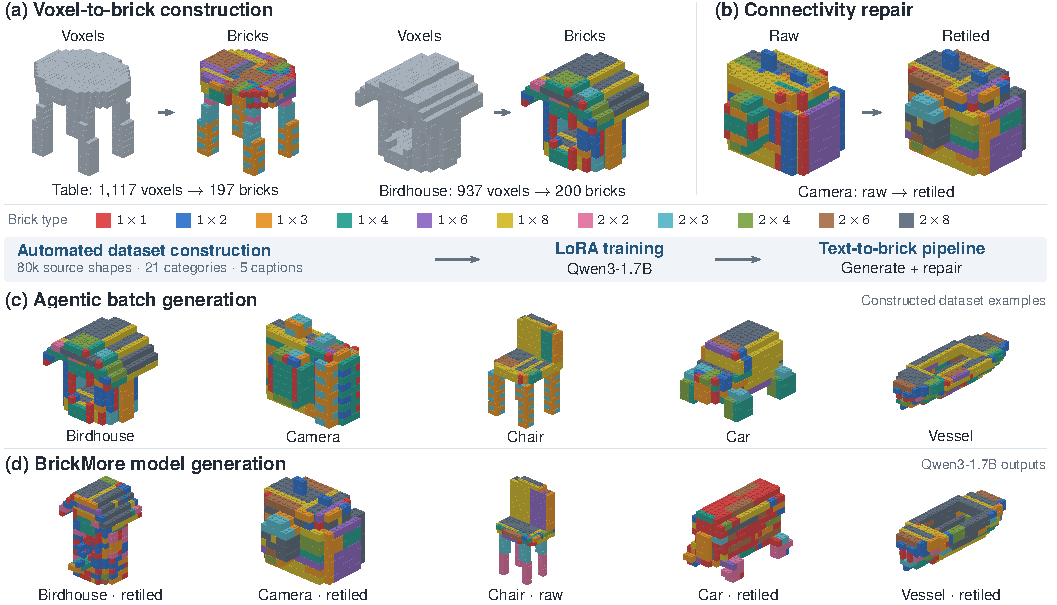
\includegraphics[width=0.74\textwidth]{figure1.pdf}
      \captionof{figure}{\textbf{BrickForma overview.} (a) Source voxels are converted into rectangular bricks. (b) Raw predictions are retiled to repair connectivity. (c) Examples from agentic batch generation of voxel data. (d) Outputs of the fine-tuned Qwen3-1.7B pipeline. Colors encode brick type independent of orientation; they are visualization labels, not predicted appearance. Voxels are shown in gray.}
      \label{fig:teaser}
    \end{center}
    \vspace{-0.2em}
  }%
}
\makeatother

\begin{document}

\maketitle


%xiao
\begin{abstract}
Geometric spatial reasoning underlies applications from robotics to automated design, yet the ability of large language models (LLMs) to turn a verbal description into a physically connected three-dimensional assembly remains largely underexplored. LEGO\textsuperscript{\tiny\textregistered} brick assembly is a demanding constructive probe of this ability: a short, underspecified prompt leaves dimensions, proportions, and part layout implicit, and a valid answer must match the semantic intent of the prompt while completing this geometry with discrete pieces that interlock through studs. We study this setting as the \texttt{Text-to-Brick} task and present BrickForma, a framework that crystallizes the geometric knowledge of large language models into a compact model for this task, \textit{without the need for human-crafted or human-verified training input}. We leverage parametric programs written with large-language-model assistance to generate 80,000 source voxel models across 21 categories on a $48^3$ grid, each described at five levels of detail, yielding approximately 400,000 caption records that tie varying amounts of language to shared geometry. A voxel-to-brick conversion pipeline with connection analysis and local retiling turns these shapes into geometrically checked brick targets, on which we fine-tune Qwen3-1.7B to predict brick dimensions and positions from text. A mixed-integer linear programming stage then seeks an exact cover of the voxel target reconstructed from these predictions with a single stud-connected component. On 114 shared prompts spanning five description levels, BrickForma achieves the highest mean VQAScore, PE, and SigLIP2 at every level, including the shortest descriptions, against the state-of-the-art approaches BrickGPT and BrickNet, while matching BrickGPT's mean invalid-placement ratio of 0.00\%. These results suggest that executable programs and checked
% Reframed abstract and introduction for BrickForma.
% All numbers and results are carried over unchanged from the previous draft.
% New citation keys to add to the .bib: legopuzzles (Tang et al., 2025, arXiv:2503.19990),
% pfp (Zhou et al., AAAI 2026, Paper Folding Puzzles), geogrambench (Luo et al., ICLR 2026).

\section{Introduction}
Spatial reasoning and geometric understanding are fundamental to human cognition and to artificial intelligence, supporting applications from robotics and navigation to computer-aided design \cite{xia2026buildarena}.
As large language models (LLMs) have matured, a growing body of work asks whether they can reason about shape, position, and transformation. Recent benchmarks probe LLMs' ability through 
%multi-step LEGO assembly~\cite{brickgpt, bricknet},
paper folding and unfolding~\cite{zhou2026paperfoldingpuzzle} and geometry expressed as procedural drawing code~\cite{luo2026geogrambench}. Each reports pronounced deficiencies in current models. These studies largely assess spatial reasoning by asking a model to select or compute an answer. A complementary and less examined question is whether a language model can \emph{construct}: given only words, can it produce a three-dimensional object whose parts are correctly sized, correctly placed, and physically joined?

%xiao: use lego instead of Brick
LEGO brick assembly makes this question concrete. A concise narrative request such as \emph{a simple chair} identifies an object category while leaving its dimensions, proportions, and part layout largely unspecified. Answering it requires three coupled forms of geometric spatial reasoning. The model must complete the missing geometry from prior knowledge of what the object looks like. It must discretize that geometry into pieces of fixed dimensions at integer positions on a grid. And it must respect the difference between spatial adjacency and stud connectivity, since pieces that touch side by side do not hold together unless they interlock vertically through studs. We refer to this setting as the \texttt{Text-to-Brick} task: the translation from a natural-language description, at any level of detail, to a set of (LEGO) brick placements that reproduces the described shape as a single connected assembly. Because every output can be checked for coverage, bounds, and connectivity, the task provides a verifiable test of whether linguistic knowledge has become spatial structure.

Prior work has established that language models can be trained for this task. BrickGPT~\cite{brickgpt} learns autoregressive brick-placement sequences and incorporates validity checks with physics-aware rollback during inference. BrickNet~\cite{bricknet} adopts a graph-based representation supporting a broader range of parts and connection types. Two questions remain open alongside these advances. \textbf{(Q1)} How well do generators translate \emph{limited} linguistic information into object geometry? In our five-level benchmark (Table~\ref{tab:level-results}), BrickNet obtains lower mean VQAScore, PE, and SigLIP2 than BrickForma at the shortest description levels, L1, a gap that only level-wise evaluation makes visible. \textbf{(Q2)} Where should the geometric knowledge needed to answer concise requests come from? Large models hold broad knowledge of object proportions and part structure, but that knowledge is implicit and their outputs carry no structural guarantee. Whether it can be transferred to a compact model in a form that can be inspected and checked has received limited attention.

We present BrickForma, which addresses both questions by \emph{crystallizing} large-model geometric knowledge into a small model through executable programs rather than through the large model's direct outputs. With GPT-6.1 Sol assistance, we develop parametric programs that vary object proportions, part dimensions, openings, and support arrangements to synthesize voxel shapes in batches.
In this form, what a large model knows about a category becomes explicit and executable: each program fixes the structure of an object family and exposes its geometric degrees of freedom as parameters, so every generated shape is exact by construction. The source collection contains 80,000 models across 21 categories on a $48^3$ grid. Each model is paired with five levels of description that progressively introduce structural, geometric, proportional, and appearance information. The resulting approximately 400,000 caption records link concise requests and detailed specifications to shared geometry, so that a model trained on them learns to supply at the shortest level the geometric details that the longest level states outright.

Turning voxel shapes into brick targets is where spatial adjacency and stud connectivity must be separated. A connected voxel volume can be tiled by pieces that touch side by side without connecting through studs. Our conversion pipeline combines same-color tiling, connection analysis, and local bridging and retiling to construct geometrically checked target layouts, with changes to source voxels recorded in derived models. The integrated dataset release includes 79,301 models passing its dataset-level geometric checks. We fine-tune Qwen3-1.7B~\cite{qwen3} ~\cite{lora} on caption--placement pairs to predict brick dimensions and spatial positions. The knowledge transfer therefore passes through three inspectable stages, from programs to checked brick layouts to a 1.7B-parameter generator, and the small model never trains on an unverified large-model output.

Geometric reconstruction complements the small model's predictions with explicit structural enforcement. From the supported, in-bounds portions of predicted placements, the pipeline forms a voxel union and uses mixed-integer linear programming to seek an exact-cover layout forming a single stud-connected component. Independent coverage and connectivity checks verify the reconstructed result. This design assigns the two halves of the task to the components suited to them: the language model decides what shape a description denotes, and the solver decides how that shape holds together.
% TODO (optional, strengthens the framing): report the fine-tuned model's raw placements
% before reconstruction, and the un-tuned Qwen3-1.7B, to isolate what crystallization contributes.

We evaluate BrickForma against BrickGPT and BrickNet on 114 shared prompts spanning five description levels. BrickForma achieves the highest mean VQAScore, PE, and SigLIP2 at every level, including the shortest descriptions, while matching BrickGPT's mean invalid-placement ratio of 0.00\%. Reporting all five levels connects the multilevel data design to an explicit assessment of how generation changes with the amount of descriptive detail, and shows that a compact model trained on crystallized geometric data remains strongest where the prompt says least.

In summary, the main contributions of this work are as follows:

\textbf{Crystallizing large-model geometric knowledge into a small model 
without human-verified data.}
We propose a data generation pipeline for transferring geometric and 
spatial knowledge from large language models to a compact model: the 
large model's knowledge is externalized as executable parametric programs, 
converted into geometrically validated training data, and distilled into 
a 1.7B-parameter model without relying on human verification. 
We demonstrate that this approach enables a small language model to 
outperform state-of-the-art methods, BrickGPT and BrickNet, by \%.
% Insert percentage here.



\textbf{A multi-level dataset that enables experimental validation of small language model alignment across 
various levels of descriptive detail.}
With our LLM-assisted parametric data construction pipeline, we generated 80,000 
source voxel models. Each voxel model is paired with five levels of textual description 
and geometrically validated brick targets. We fine-tuned Qwen3-1.7B on this dataset and carried out level-wise evaluation 
against BrickGPT and BrickNet assesses text--image alignment and invalid 
placements across descriptions ranging from concise prompts to detailed 
specifications. BrickForma consistently achieves the highest mean 
alignment scores across all five levels.
% \begin{abstract}
    Text-to-brick generation requires translating natural-language descriptions into spatial arrangements of discrete pieces. Concise prompts leave object dimensions, proportions, and part layouts implicit, making geometric data construction and structural constraints central to this task. We present BrickForma, a framework combining voxel-to-brick data construction, language-model fine-tuning, and geometric reconstruction. LLM-assisted parametric programs generate 80,000 source voxel models across 21 categories on a $48^3$ grid, each paired with five levels of description. The resulting approximately 400,000 caption records link varying amounts of linguistic detail to shared object geometry. A conversion pipeline integrates same-color tiling, connection analysis, and local bridging and retiling to construct geometrically checked brick targets. We fine-tune Qwen3-1.7B with low-rank adaptation on caption--placement pairs to predict brick dimensions and positions from text. A subsequent reconstruction stage uses mixed-integer linear programming to seek an exact cover of the reconstructed voxel target with a single stud-connected component. Experiments compare BrickForma with BrickGPT and BrickNet on 114 shared prompts spanning five description levels. Under a common rendering protocol, BrickForma achieves the highest mean VQAScore, PE, and SigLIP2 at every level, including the shortest descriptions, while matching BrickGPT's mean invalid-placement ratio of 0.00\%.
\end{abstract}


% \section{Introduction}
Text-to-brick generation connects natural-language descriptions with the spatial arrangement of discrete building pieces. A concise request such as \emph{a simple chair} identifies an object category while leaving its dimensions, proportions, and part layout largely unspecified. A generator must complete these geometric details and express the resulting shape through brick placements. Addressing this challenge involves both text--geometry supervision spanning different amounts of descriptive information and explicit constraints governing how discrete pieces connect.

BrickGPT~\cite{brickgpt} learns autoregressive brick-placement sequences and incorporates validity checks with physics-aware rollback during inference. BrickNet~\cite{bricknet} adopts a graph-based representation supporting a broader range of parts and connection types. Alongside these advances, generation from concise descriptions warrants explicit examination. In our five-level benchmark (Table~\ref{tab:level-results}), BrickNet obtains lower mean VQAScore, PE, and SigLIP2 than BrickForma at the two shortest description levels, L1 and L2. This observed gap motivates a closer examination of how generators translate limited linguistic information into object geometry. Level-wise evaluation makes performance on concise requests visible alongside performance on detailed specifications.

We present BrickForma, placing programmatic geometric data construction at the foundation of text-conditioned brick generation. With large-language-model assistance, we develop parametric programs that vary object proportions, part dimensions, openings, and support arrangements to synthesize voxel shapes in batches. The source collection contains 80,000 models across 21 categories on a $48^3$ grid. Each model is paired with five levels of bilingual description that progressively introduce structural, geometric, proportional, and appearance information. These approximately 400,000 caption records link concise requests and detailed specifications to shared geometry, providing multilevel supervision for text-conditioned spatial layout prediction.

Converting voxel shapes into brick targets explicitly addresses the distinction between spatial adjacency and stud connectivity. A connected voxel volume can be tiled by pieces that touch side by side without connecting through studs. Our conversion pipeline combines same-color tiling, connection analysis, and local bridging and retiling to construct geometrically checked target layouts, with changes to source voxels recorded in derived models. The integrated dataset release includes 79,301 models passing its dataset-level geometric checks. We fine-tune Qwen3-1.7B~\cite{qwen3} with low-rank adaptation~\cite{lora} on caption--placement pairs to predict brick dimensions and spatial positions.

Geometric reconstruction complements the language model's placement predictions. From the supported, in-bounds portions of predicted placements, the pipeline forms a voxel union and uses mixed-integer linear programming to seek an exact-cover layout forming a single stud-connected component. Independent coverage and connectivity checks verify the reconstructed result. This design decouples text-conditioned shape prediction in the language model from explicit structural enforcement in the reconstruction stage.

We evaluate BrickForma against BrickGPT and BrickNet on 114 shared prompts spanning five description levels. BrickForma achieves the highest mean VQAScore, PE, and SigLIP2 at every level, including the shortest descriptions, while matching BrickGPT's mean invalid-placement ratio of 0.00\%. Reporting all five levels connects the framework's multilevel data design to an explicit assessment of generation across different amounts of descriptive detail.

Our contributions are:
\begin{enumerate}
\item An LLM-assisted parametric data-construction pipeline producing 80,000 source voxel models with five levels of associated description, linking varying amounts of linguistic detail to shared object geometry.
\item A text-to-brick framework integrating voxel-to-brick target construction, Qwen3-1.7B fine-tuning, and MILP-based exact-cover reconstruction with independent coverage and stud-connectivity checks.
\item A five-level evaluation against BrickGPT and BrickNet that explicitly examines concise descriptions alongside detailed specifications through text--image alignment and invalid-placement measurements.
\end{enumerate}

%xiao

\begin{figure*}[t]
\centering
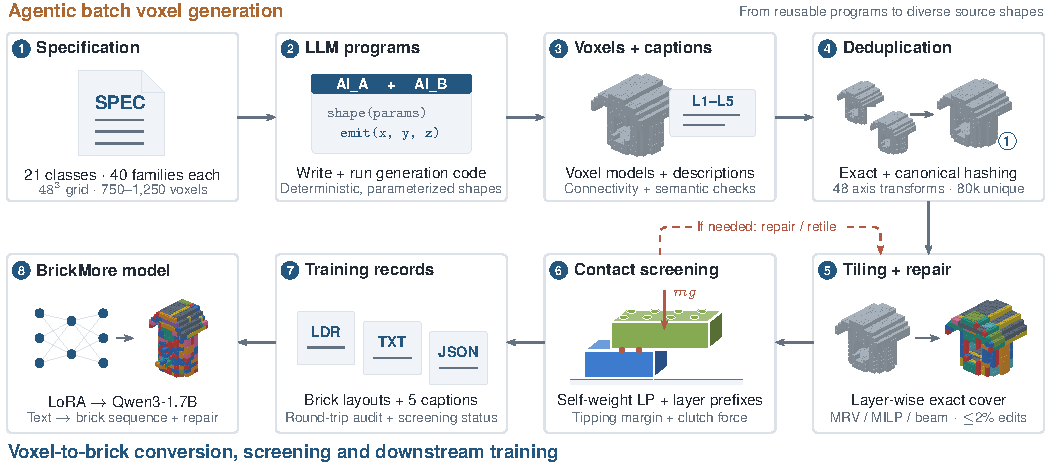
\includegraphics[width=0.94\textwidth]{figure2.pdf}
\caption{\textbf{Data-construction workflow.} Parametric programs written by GPT-6.1 Sol through agentic batch generation produce voxel shapes and captions, followed by deduplication, voxel-to-brick tiling, repair, contact-based screening, and audited export for fine-tuning. The dashed arrow denotes repair or retiling when needed. Screening is distinct from a guarantee of physical stability. Brick colors follow the legend in Figure~\ref{fig:teaser}.}
\label{fig:data-workflow}
\end{figure*}

\section{Related Work}
\paragraph{Brick assembly and generation.}
Learning-based brick construction has been studied as graph generation~\cite{thompson2020lego}, as combinatorial construction with deep reinforcement learning~\cite{brickbybrick}, and as interactive structural understanding in a LEGO simulator~\cite{breakandmake}. For text-conditioned generation, BrickGPT represents a design as an autoregressively generated sequence of brick placements and uses brick-level rejection sampling with physics-aware rollback at inference~\cite{brickgpt}; BrickNet represents part connectivity through a graph-backed parametrization and trains autoregressive models on its assembly sequences~\cite{bricknet}. BrickForma also generates placement sequences from text, on a larger $48^3$ grid with a 20-type library, and examines geometric reconstruction and connectivity in a separate post-generation stage.

\paragraph{Stability analysis.}
StableLego analyzes the structural stability of block-stacking assemblies with a force-balance optimization~\cite{stablelego}. Such analyses depend on their mechanical assumptions. In BrickForma, geometric connectivity and the contact-based screening in the dataset materials address different properties; neither alone establishes that every generated model can be physically assembled and remains stable.

\paragraph{Procedural data and parameter-efficient fine-tuning.}
Procedural generation is a common way to obtain large, controllable 3D training data~\cite{infinigen}. BrickForma uses a language model to write the procedural generators rather than to emit coordinates directly. The generator itself is adapted with LoRA~\cite{lora}, following the BrickGPT recipe of fine-tuning a pretrained language model on serialized brick sequences~\cite{brickgpt}.

\section{Dataset Construction}
\label{sec:dataset}
\subsection{Parametric Voxel Generation}
BrickMore-48 contains 80,000 voxel models on a $48^3$ grid across 21 categories (3,805--3,810 per category), each paired with five bilingual captions at levels L1 (concise) to L5 (detailed). The models are produced by parametric generator programs written through agentic batch generation with GPT-6.1 Sol; the programs, rather than the language model itself, emit the voxel coordinates. Each record includes a geometry plan and a dataset version identifier for reproduction, and exact and canonical (48 axis/sign transforms) occupancy hashes show no duplicates across the two 40,000-model shards. Figure~\ref{fig:data-workflow} summarizes the workflow; sample shapes are shown in Appendix~\ref{app:dataset}.


\subsection{Voxel-to-Brick Conversion and Checks}
The conversion pipeline tiles occupied voxels with same-color rectangular bricks and analyzes their connections. Local bridging and retiling address ungrounded components, and changes to source voxels are recorded separately. Each converted model carries a \texttt{validation.json} that records three geometric constraints: the occupied voxels form a single six-neighbour connected component, every brick component is grounded, and the bricks exactly cover the (derived) target voxels. Under these release rules a layout may consist of several brick components that are each grounded; this criterion differs from the single stud-connected component enforced by post-generation retiling (Section~\ref{sec:model}). The dataset materials also describe a contact-based gravity screening procedure; its outputs are screening results under stated assumptions rather than proof of physical stability (Appendix~\ref{app:dataset}); training-data selection uses the geometric checks.

\subsection{Integrated Release and Training Corpus}
The full retile release records 79,298 geometrically passing models; the 702 failures (0.88\%) are concentrated in table (132), bookshelf (110), vessel (89), bowl (79), and bus (75). Replacing all 1,905 batch-B piano slots (1,902 passing) with a regenerated release in which all 1,905 pass gives an integrated count of $79{,}298-1{,}902+1{,}905=79{,}301$ passing models. This number is computed from the two release reports, not from a new full-dataset verification run, and the original A/B download does not apply the replacement automatically. Fine-tuning uses only geometrically passing models (Table~\ref{tab:training-data}).

\begin{table}[t]
\centering
\small
\setlength{\tabcolsep}{4pt}
\begin{tabular}{lr}
\toprule
Item & Count \\
\midrule
Source models / categories / grid & 80,000 / 21 / $48^3$ \\
Bilingual caption records & 400,000 \\
Failing in full retile release & 702 (0.88\%) \\
Passing in full retile release & 79,298 \\
Piano models restored by revised release & 3 \\
Integrated passing models & 79,301 \\
(model, English caption) samples & 396,610 \\ % TODO verify sample count (待用户确认)
Training / validation samples & 356,955 / 39,655 \\
Tokens over 3 epochs & 2,228,044,818 \\ % TODO verify token count (待用户确认; model card says ~2.19B)
\bottomrule
\end{tabular}
\caption{Dataset and fine-tuning corpus.}
\label{tab:training-data}
\end{table}
% TODO verify sample count (待用户确认)
% 79,301 models x 5 captions = 396,505, which differs from the reported 396,610 by 105.
% A released model card states "79,322 models x 5 captions = 396,610 samples" and "~2.19B tokens total";
% these conflict with the 79,301 integrated count and with 2,228,044,818 tokens.
% trainer_state.json / build_stats.json were not found. Do not resolve without user confirmation.

\section{BrickForma Text-to-Brick Model}
\label{sec:model}
\subsection{Fine-Tuning}
\label{sec:training}
We fine-tune Qwen3-1.7B on BrickMore-48 with a library of 20 brick types. Relative to StableText2Brick used by BrickGPT ($20^3$, 14 types), the library adds six footprints ($3{\times}2$, $2{\times}3$, $3{\times}1$, $1{\times}3$, $2{\times}8$, $8{\times}2$). Each object occupies 750--1,250 voxels with coordinates in $\{0,\ldots,47\}$. Training uses only the English captions (\texttt{captionEn}, L1--L5); the Chinese captions are not used. Samples are split by model at a 9:1 ratio, so the captions of one model never straddle the split.

Each sample is a three-turn chat, structurally identical to the official BrickGPT data-preparation script: a system prompt (``You are a helpful assistant.''), a user instruction adapted to the $48^3$ world that lists the 20 allowed dimensions, and an assistant reply with one brick per line, e.g.\ $2{\times}4\ (x,y,z)$. No thinking content is used; inference sets \texttt{enable\_thinking=False} to match training. Brick dimensions are serialized Y-first, then X, which differs from the StableText2Brick convention; training and inference share this convention, and downstream parsers must restore the orientation consistently.

Hyperparameters follow the Qwen3 fine-tuning script in the official BrickGPT repository (Table~\ref{tab:finetune-config}) rather than the LLaMA numbers in the original paper; Appendix~\ref{app:training} compares the two. Sequences are unpacked so that each caption--sequence boundary is preserved, and dependencies are pinned to the official TRL~0.17 stack. Training runs 133,860 steps in 25.3 hours ($\approx$202 GPU-hours). Validation loss, computed every 500 steps on a 2,000-sample validation subset, reaches its minimum of 0.0308 at step 79,000 (epoch 1.77) and rises to 0.0339 by the end of epoch 3. Because \texttt{load\_best\_model\_at\_end} is enabled, the released weights are those of step 79,000, so the additional third epoch does not degrade the released model. Full loss curves are listed in Appendix~\ref{app:training}.

\begin{table}[t]
\centering
\small
\setlength{\tabcolsep}{3pt}
\begin{tabular}{@{}l>{\raggedright\arraybackslash}p{0.58\linewidth}@{}}
\toprule
Item & Value \\
\midrule
Base model & Qwen3-1.7B (bf16) \\
Adaptation & LoRA, $r=16$, $\alpha=32$, dropout $0.05$, all linear layers \\
Optimization & LR $10^{-4}$, cosine, 100 warm-up steps, 3 epochs \\
Batch / max length & effective 8 (8 GPUs $\times$ 1) / 8,192 \\
Hardware & DDP, 8$\times$RTX 4090D (24\,GB) \\
Released checkpoint & step 79,000 (best validation loss) \\
Software & transformers 4.51.3, trl 0.17.0, peft 0.15.2 \\
\bottomrule
\end{tabular}
\caption{Fine-tuning configuration (details in Appendix~\ref{app:training}).}
\label{tab:finetune-config}
\end{table}

\begin{figure*}[t]
\centering
\setlength{\tabcolsep}{3pt}
\begin{tabular}{@{}ccc@{}}
\textbf{BrickForma} & \textbf{BrickGPT} & \textbf{BrickNet} \\
\multicolumn{3}{@{}p{0.96\textwidth}@{}}{\small \textbf{(a) L1:} \emph{A simple chair.}} \\
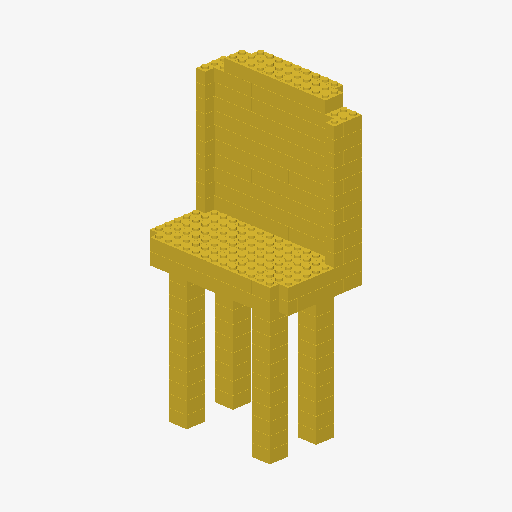
\includegraphics[width=0.136\textwidth]{figures/short_prompts/source/brickmore__chair-L1-A__stitched/01.png}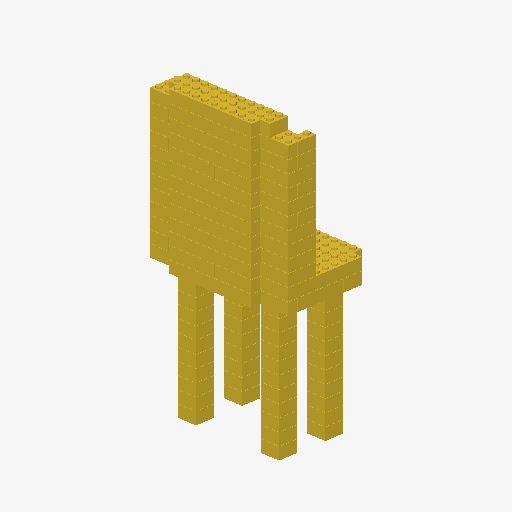
\includegraphics[width=0.136\textwidth]{figures/short_prompts/source/brickmore__chair-L1-A__stitched/05.png} & 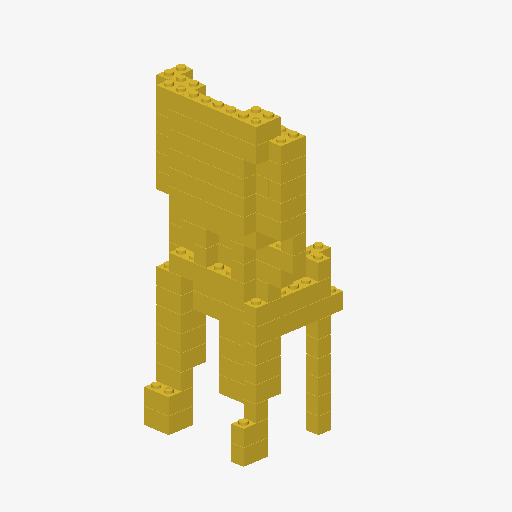
\includegraphics[width=0.136\textwidth]{figures/short_prompts/source/brickgpt__chair_L1_P01__generated/01.png}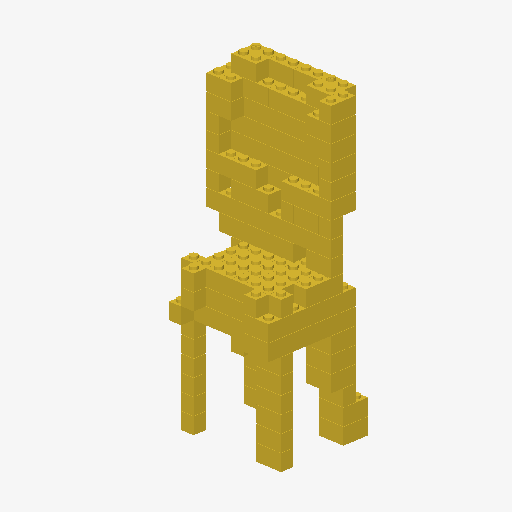
\includegraphics[width=0.136\textwidth]{figures/short_prompts/source/brickgpt__chair_L1_P01__generated/05.png} & 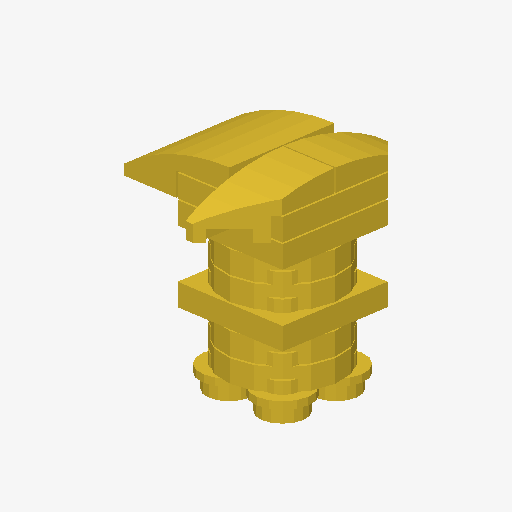
\includegraphics[width=0.136\textwidth]{figures/short_prompts/source/bricknet__chair_L1_P01__generated/01.png}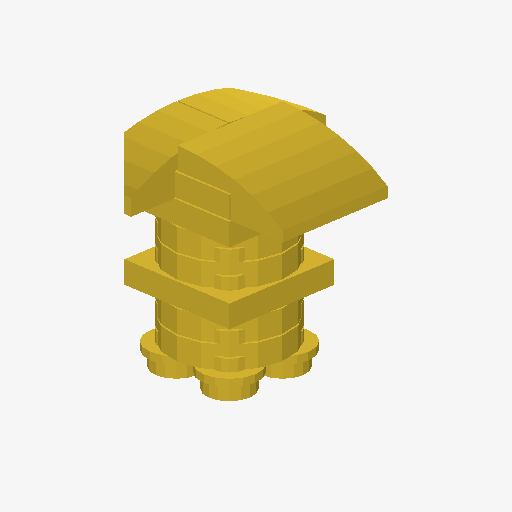
\includegraphics[width=0.136\textwidth]{figures/short_prompts/source/bricknet__chair_L1_P01__generated/05.png} \\[0pt]
\multicolumn{3}{@{}p{0.96\textwidth}@{}}{\small \textbf{(b) L1:} \emph{A compact four-door car.}} \\
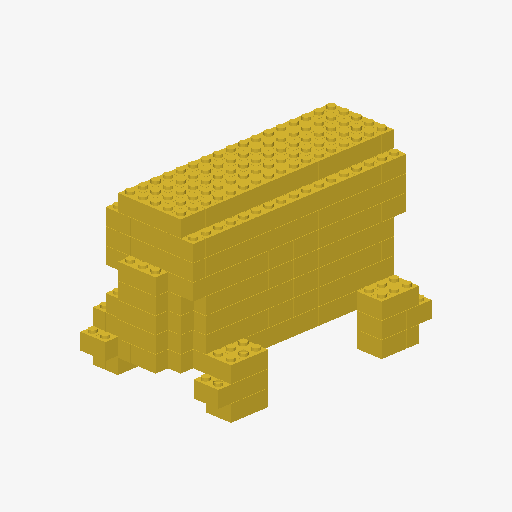
\includegraphics[width=0.136\textwidth]{figures/short_prompts/source/brickmore__car-L1V2__stitched/01.png}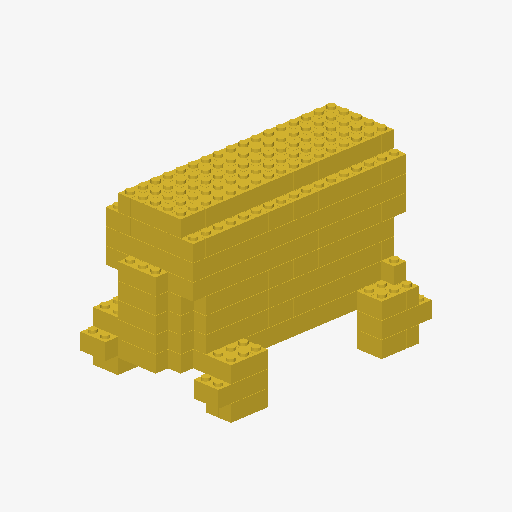
\includegraphics[width=0.136\textwidth]{figures/short_prompts/source/brickmore__car-L1V2__stitched/05.png} & 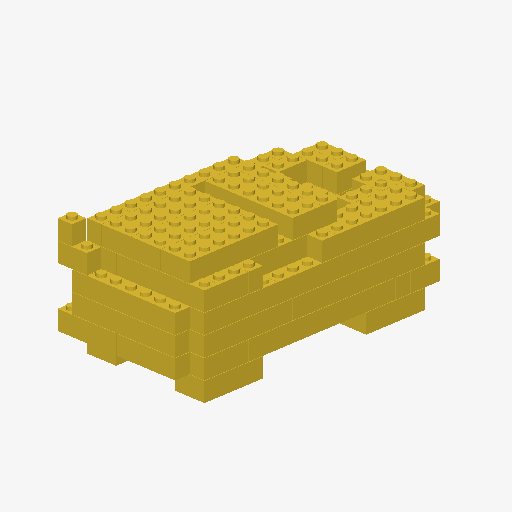
\includegraphics[width=0.136\textwidth]{figures/short_prompts/source/brickgpt__car_L1_P01__generated/01.png}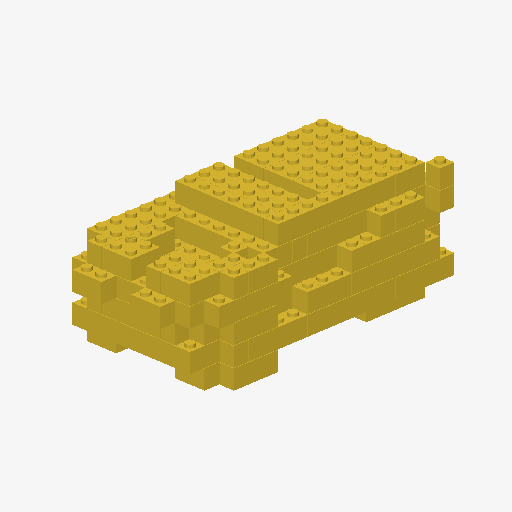
\includegraphics[width=0.136\textwidth]{figures/short_prompts/source/brickgpt__car_L1_P01__generated/05.png} & 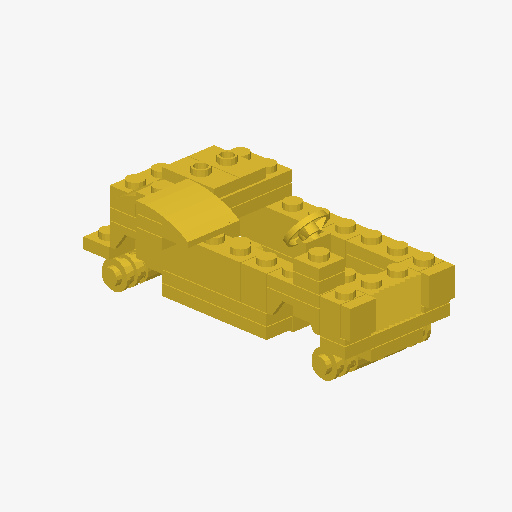
\includegraphics[width=0.136\textwidth]{figures/short_prompts/source/bricknet__car_L1_P01__generated/01.png}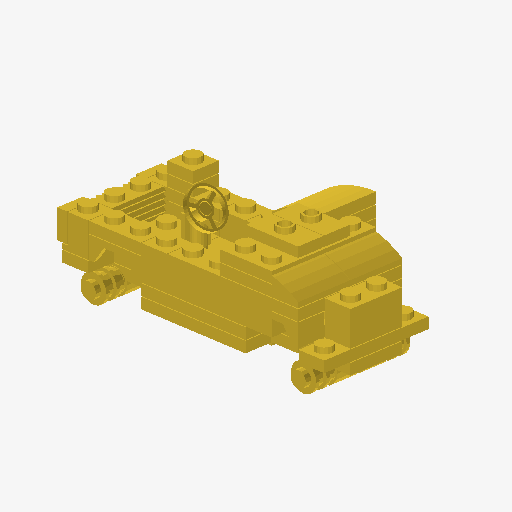
\includegraphics[width=0.136\textwidth]{figures/short_prompts/source/bricknet__car_L1_P01__generated/05.png} \\[0pt]
\multicolumn{3}{@{}p{0.96\textwidth}@{}}{\small \textbf{(c) L2:} \emph{A straight bench with a plank top and chunky leg blocks.}} \\
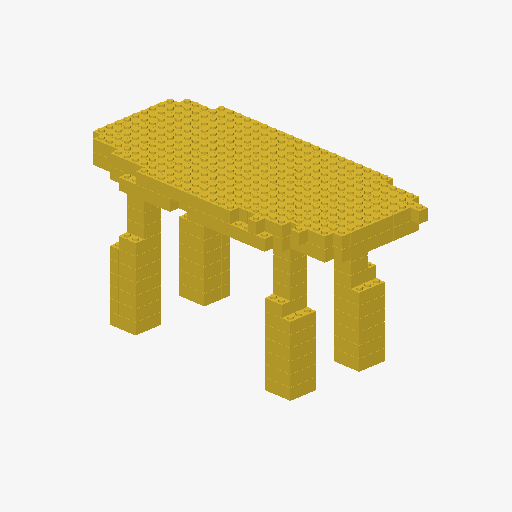
\includegraphics[width=0.136\textwidth]{figures/short_prompts/source/brickmore__bench-L2V4__stitched/01.png}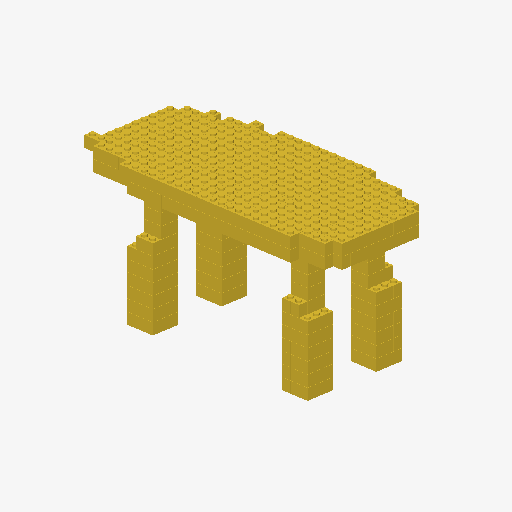
\includegraphics[width=0.136\textwidth]{figures/short_prompts/source/brickmore__bench-L2V4__stitched/05.png} & 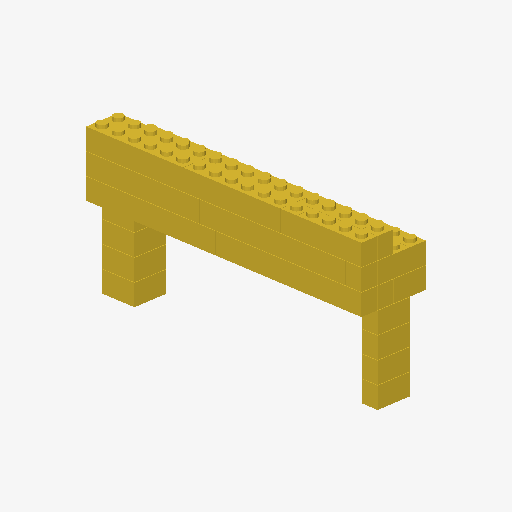
\includegraphics[width=0.136\textwidth]{figures/short_prompts/source/brickgpt__bench_L2_P01__generated/01.png}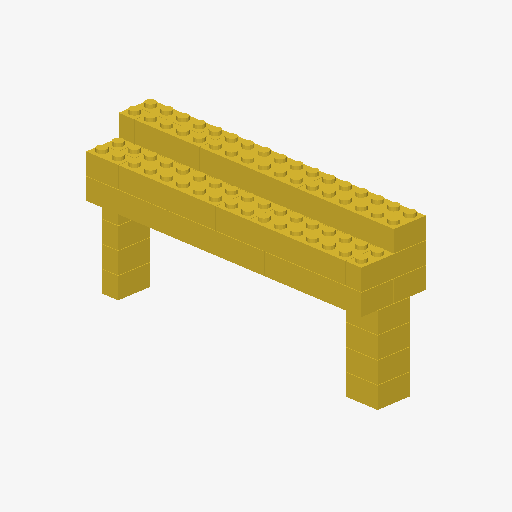
\includegraphics[width=0.136\textwidth]{figures/short_prompts/source/brickgpt__bench_L2_P01__generated/05.png} & 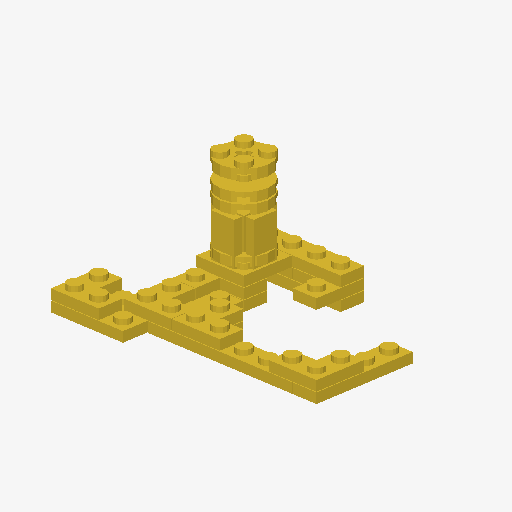
\includegraphics[width=0.136\textwidth]{figures/short_prompts/source/bricknet__bench_L2_P01__generated/01.png}
\includegraphics[width=0.136\textwidth]{figures/short_prompts/source/bricknet__bench_L2_P01__generated/05.png} \\[0pt]
\multicolumn{3}{@{}p{0.96\textwidth}@{}}{\small \textbf{(d) L2:} \emph{A rounded camera carries a circular lens at the front. The barrel connects to its body, the grip is on the right side, and the shutter and viewfinder sit on top.}} \\
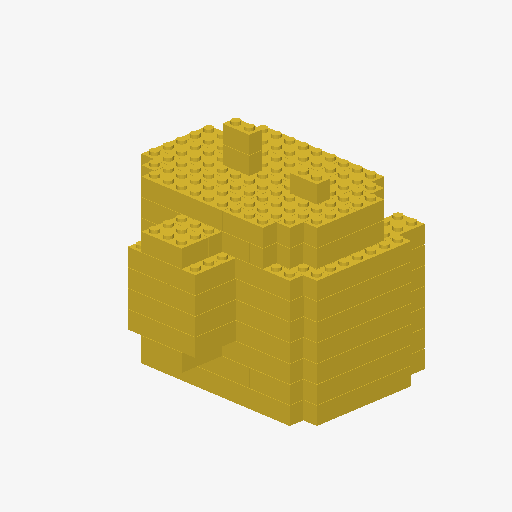
\includegraphics[width=0.136\textwidth]{figures/short_prompts/source/brickmore__camera_L2_P1_G__stitched/01.png}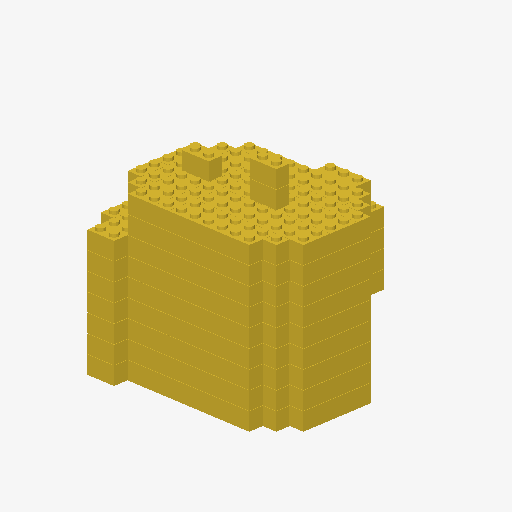
\includegraphics[width=0.136\textwidth]{figures/short_prompts/source/brickmore__camera_L2_P1_G__stitched/05.png} & 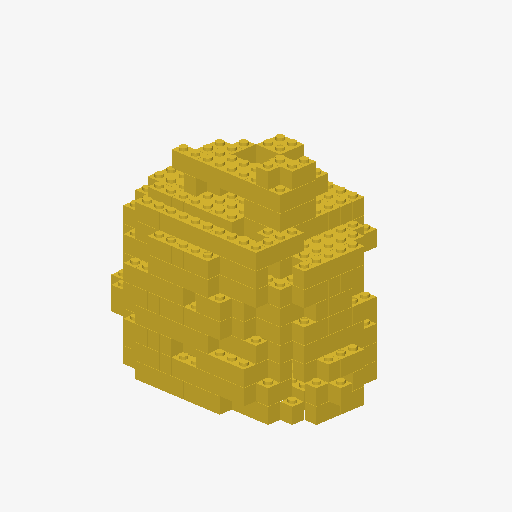
\includegraphics[width=0.136\textwidth]{figures/short_prompts/source/brickgpt__camera_L2_P01__generated/01.png}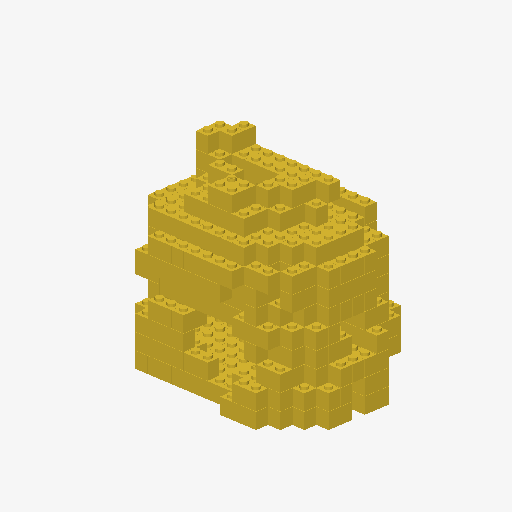
\includegraphics[width=0.136\textwidth]{figures/short_prompts/source/brickgpt__camera_L2_P01__generated/05.png} & 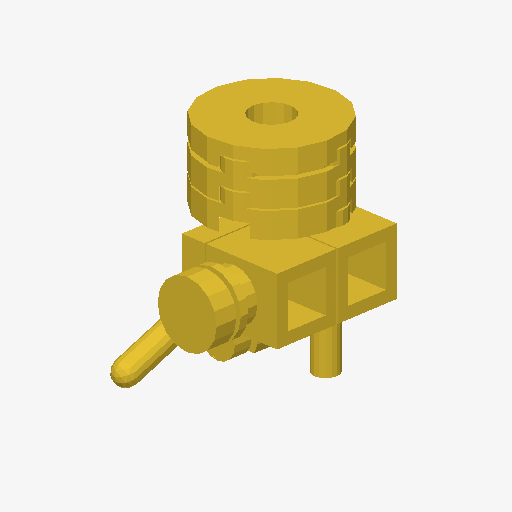
\includegraphics[width=0.136\textwidth]{figures/short_prompts/source/bricknet__camera_L2_P01__generated/01.png}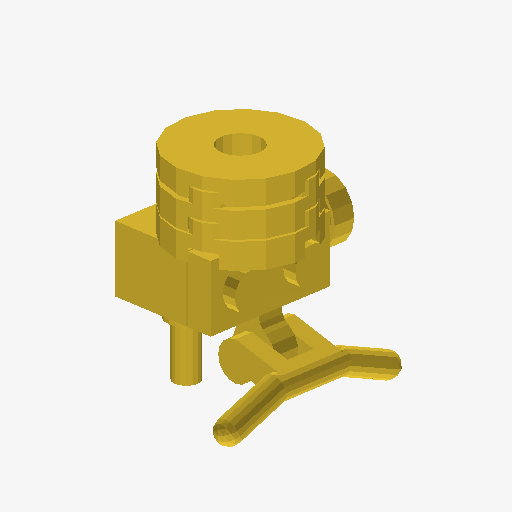
\includegraphics[width=0.136\textwidth]{figures/short_prompts/source/bricknet__camera_L2_P01__generated/05.png} \\[0pt]
\end{tabular}
\caption{Matched short-prompt examples from the main comparison. Each row uses the same prompt across all three systems and displays the same two archived camera azimuths ($45^\circ$, $225^\circ$), with $25^\circ$ elevation and uniform yellow rendering. BrickForma uses the fixed retiled main-comparison output in these four cases. Chair and bench illustrate higher BrickForma VQAScore; car and camera retain counterexamples where BrickNet has a higher VQAScore. Examples illustrate variation across cases and do not estimate a success rate.}
\label{fig:short-prompts}
\end{figure*}


\subsection{Inference and Retiling}
Inference follows the seed-escalation and repair procedure in Algorithm~\ref{alg:inference-retiling}. The model samples a placement sequence with thinking disabled, temperature $0.7$, top-$p$ $0.9$, and at most $8192$ new tokens, using seeds $42$, $104$, and $2026$ in order. A candidate is accepted when generation completes (ends with an end-of-sequence token) and the geometry validator reports no errors. Otherwise, the pipeline keeps the completed draft with the fewest validator error records $\mathrm{Err}(\cdot)$ (line format, library membership, bounds, and overlaps). It then forms the voxel union $C$ of the in-bounds cells of supported library placements, solves a shape-preserving exact cover of $C$ with a single stud-connected component by MILP under a $12$--$60$--$180$\,s time ladder, and audits the result independently. If no cover is found within this budget, the raw draft is retained and a new seed may be queued. A separate recovery path may extend the budget to $600$\,s and sample seeds outside $S$; it is not part of the default loop. We call the MILP output the \emph{retiled} layout (files are named \texttt{stitched}) and the model's draft the \emph{raw} layout.

\begin{algorithm}[t]
\caption{BrickForma inference and retiling}
\label{alg:inference-retiling}
\small
\begin{algorithmic}[1]
\REQUIRE prompt $c$; fine-tuned model $\theta$; library $\mathcal{L}$ (20 types); seeds $S=(42,104,2026)$; MILP tiers $T=(12,60,180)$\,s
\ENSURE $(B_{\mathrm{out}}, \textit{status})$, $\textit{status}\in\{\textsc{Success},\textsc{Draft},\textsc{Failed}\}$
\STATE $B \gets \emptyset$; $A \gets \emptyset$
\FOR{$s \in S$}
  \STATE $(B_s,\textit{rep}) \gets \mathrm{Parse}(\theta.\mathrm{Generate}(c,\ \mathrm{seed}{=}s))$
  \STATE $A \gets A \cup \{(B_s,\textit{rep})\}$
  \IF{$\textit{rep}.\mathrm{complete} \land \textit{rep}.\mathrm{valid}$}
    \STATE $B \gets B_s$; \textbf{break}
  \ENDIF
\ENDFOR
\IF{$B=\emptyset$}
  \IF{no completed draft in $A$}
    \RETURN $(\emptyset,\ \textsc{Failed})$
  \ENDIF
  \STATE $B \gets \arg\min_{\text{completed } a\in A} \mathrm{Err}(a)$
\ENDIF
\STATE $C \gets \mathrm{UnionVoxels}(B;\ \mathcal{L},\ 48^3)$ \COMMENT{clip; overlaps count once}
\FOR{$\tau \in T$}
  \STATE $B^{*} \gets \mathrm{MILP\text{-}SingleStudCover}(C,\ \tau)$
  \IF{$B^{*}\neq\emptyset$}
    \STATE $\mathrm{Audit}(B^{*},C)$ \COMMENT{one stud component, $\mathrm{voxels}(B^{*}){=}C$}
    \RETURN $(B^{*},\ \textsc{Success})$
  \ENDIF
\ENDFOR
\STATE $\mathrm{QueueReseed}(c)$
\RETURN $(B,\ \textsc{Draft})$ \COMMENT{unsolved: keep raw draft}
\end{algorithmic}
\end{algorithm}

\section{Comparative Evaluation}
\label{sec:eval}
\subsection{Setup and Metrics}
We compare the provided outputs of BrickForma, BrickGPT, and BrickNet on 114 shared prompts covering 21 categories and five description levels (one output per system and prompt). For BrickForma, the provided output is the first candidate, using the retiled layout when available: 110 of the 114 outputs are retiled and 4 are raw. All systems are rendered with the same protocol: uniform yellow material, $512{\times}512$ orthographic views at $25^{\circ}$ elevation and eight azimuths ($0^{\circ}$ to $315^{\circ}$ in $45^{\circ}$ steps).

\emph{Text--image alignment.} VQAScore~\cite{vqascore} is the probability that Qwen2.5-VL-7B-Instruct~\cite{qwen25vl} answers ``Yes'' to whether a rendered view shows the prompt. PE and SigLIP2 are image--text matching scores from PE-Core-bigG-14-448~\cite{pe} and SigLIP2 giant-opt-patch16-384~\cite{siglip2}, whose text encoders read at most 72 and 64 tokens, respectively. For each metric, a model's score is the maximum over its eight views, then averaged over prompts.

\emph{Invalid placements.} For a model with placements $b_1,\ldots,b_n$ in exported file order,
\begin{equation}
P_{\mathrm{inv}} = \frac{1}{n}\sum_{i=1}^{n}\mathbf{1}\big[\,b_i \text{ is invalid given } b_1,\ldots,b_{i-1}\big],
\end{equation}
where invalidity (e.g.\ intersection with earlier parts) is decided by BrickNet's original inset collision kernel~\cite{bricknet}. We report the macro average over models. The original generation order is not verified, and a zero $P_{\mathrm{inv}}$ does not certify stud connectivity, stability, or buildability.

The systems differ in candidate selection, filtering, and post-processing; the comparison characterizes these delivered outputs rather than isolated model capability.

% Generated by scripts/build_level_results.py; edit the input data and rebuild.
% GitHub source commit: dfe1c94fc86b722247ed5c8208011313f535c5ec
\begin{table*}[t]
\centering
\small
\setlength{\tabcolsep}{5pt}
\begin{tabular}{lrrlrrrr}
\toprule
Level & $n$ & Words & System & $P_{\mathrm{inv}}\downarrow$ & VQA$\uparrow$ & PE$\uparrow$ & SigLIP2$\uparrow$ \\
\midrule
L1 & 21 & 7.8 & BrickForma & \textbf{0.00\%} & \textbf{0.2201} & \textbf{0.1693} & \textbf{0.0478} \\
 & & & BrickGPT & \textbf{0.00\%} & 0.1085 & 0.1364 & 0.0173 \\
 & & & BrickNet & 14.83\% & 0.0833 & 0.1151 & 0.0035 \\
\midrule
L2 & 21 & 17.3 & BrickForma & \textbf{0.00\%} & \textbf{0.3615} & \textbf{0.1763} & \textbf{0.1027} \\
 & & & BrickGPT & \textbf{0.00\%} & 0.2507 & 0.1415 & 0.0331 \\
 & & & BrickNet & 21.79\% & 0.0283 & 0.1178 & 0.0135 \\
\midrule
L3 & 23 & 25.8 & BrickForma & \textbf{0.00\%} & \textbf{0.2364} & \textbf{0.1839} & \textbf{0.1386} \\
 & & & BrickGPT & \textbf{0.00\%} & 0.1711 & 0.1433 & 0.0376 \\
 & & & BrickNet & 22.70\% & 0.0714 & 0.1301 & 0.0126 \\
\midrule
L4 & 25 & 41.1 & BrickForma & \textbf{0.00\%} & \textbf{0.1935} & \textbf{0.2000} & \textbf{0.1682} \\
 & & & BrickGPT & \textbf{0.00\%} & 0.1078 & 0.1535 & 0.0302 \\
 & & & BrickNet & 25.84\% & 0.0902 & 0.1475 & 0.0176 \\
\midrule
L5 & 24 & 59.6 & BrickForma & \textbf{0.00\%} & \textbf{0.0968} & \textbf{0.1947} & \textbf{0.1447} \\
 & & & BrickGPT & \textbf{0.00\%} & 0.0748 & 0.1519 & 0.0293 \\
 & & & BrickNet & 23.72\% & 0.0363 & 0.1363 & 0.0023 \\
\bottomrule
\end{tabular}
\caption{Comparison across five description levels on 114 matched prompts. $n$ is the number of prompts per system; Words is the mean English word count. $P_{\mathrm{inv}}$ is the mean per-model invalid-placement ratio, shown as a percentage. Bold marks the best mean within each level, including ties. Higher text--image scores and lower $P_{\mathrm{inv}}$ are better.}
\label{tab:level-results}
\end{table*}


\subsection{Main Results}
\begin{table}[t]
\centering
\small
\setlength{\tabcolsep}{4pt}
\begin{tabular}{lrrrr}
\toprule
System & $P_{\mathrm{inv}}$ $\downarrow$ & VQA $\uparrow$ & PE $\uparrow$ & SigLIP2 $\uparrow$ \\
\midrule
BrickForma & 0.00\% & \textbf{0.2176} & \textbf{0.1856} & \textbf{0.1231} \\
BrickGPT & 0.00\% & 0.1401 & 0.1457 & 0.0297 \\
BrickNet & 21.99\% & 0.0624 & 0.1302 & 0.0100 \\
\bottomrule
\end{tabular}
\caption{Main comparison on 114 matched prompts (means).}
\label{tab:main}
\end{table}
On these outputs, BrickForma has the highest mean on each alignment metric (Table~\ref{tab:main}). BrickForma and BrickGPT both have a mean $P_{\mathrm{inv}}$ of 0.00\%, so this measure does not distinguish them. Per prompt, BrickForma scores higher than BrickGPT on 91, 95, and 91 of 114 prompts for VQAScore, PE, and SigLIP2, respectively; no significance test is reported. The mean part counts are 413.0 (BrickForma), 152.3 (BrickGPT), and 23.3 (BrickNet); these differences should be considered when interpreting the scores, and part count alone does not measure quality. Qualitative outputs are shown in Figures~\ref{fig:teaser} and~\ref{fig:short-prompts}; historical qualitative material is in Appendix~\ref{app:eval}.

\subsection{Performance across Description Levels}
Table~\ref{tab:level-results} separates the 114-prompt comparison into five description levels. The shortest level, L1, contains 21 prompts averaging 7.8 English words. BrickForma has the highest mean VQAScore, PE, and SigLIP2 at both L1 and L2, and also leads these three metrics at each of the remaining levels. BrickForma and BrickGPT have a mean $P_{\mathrm{inv}}$ of 0.00\% at every level. The results make the short-description comparison explicit while retaining performance on richer specifications. Figure~\ref{fig:short-prompts} shows two L1 and two L2 examples with matched prompts and fixed camera views. The chair and bench cases favor BrickForma on VQAScore, while car and camera retain cases favoring BrickNet; the gallery illustrates case variation alongside the aggregate results.

\subsection{Raw versus Retiled Outputs}
\begin{table}[t]
\centering
\small
\begin{tabular}{lrr}
\toprule
Metric & Raw & Retiled \\
\midrule
$P_{\mathrm{inv}}$ $\downarrow$ & 0.1897\% & 0.0000\% \\
VQAScore $\uparrow$ & 0.2065 & 0.2071 \\
PE $\uparrow$ & 0.1858 & 0.1859 \\
SigLIP2 $\uparrow$ & 0.1379 & 0.1261 \\
Mean parts & 178.7 & 421.2 \\
\bottomrule
\end{tabular}
\caption{The 110 retiled outputs of the main comparison paired with their raw drafts (same prompt, model identifier, and caption).}
\label{tab:raw-retiled}
\end{table}
For the 110 prompts whose main-comparison output is retiled, we pair the retiled layout with its raw draft (Table~\ref{tab:raw-retiled}). Retiling reduces the mean invalid-placement ratio to zero and more than doubles the mean part count. VQAScore and PE change only slightly, while the mean SigLIP2 score decreases. These are descriptive results for this subset and do not establish a general causal effect.

\subsection{Geometric Reconstruction Audit}
\begin{table}[t]
\centering\small
\begin{tabular}{lrr}
\toprule
Geometric measure & Raw & Retiled \\
\midrule
Single stud component & 18/110 & 110/110 \\
Mean stud components & 4.29 & 1.00 \\
No body-cell overlaps & 100/110 & 110/110 \\
\midrule
\multicolumn{3}{l}{Equal voxel unions after translation: 110/110} \\
\bottomrule
\end{tabular}
\caption{Independent export-geometry audit of the 110 matched raw/retiled pairs. Equality compares occupied voxel unions after translation normalization.}
\label{tab:reconstruction-geometry}
\end{table}

We independently audit the exported rectangular-brick placements for the same 110 pairs (Table~\ref{tab:reconstruction-geometry}). A stud-contact edge joins bricks on adjacent layers when their footprints share at least one stud cell; lateral contact alone does not create an edge. Placements are mapped to a grid with 20 LDU horizontal pitch and 24 LDU layer height. Each export is translated to a common occupied-cell origin before voxel-union comparison, accommodating small export-coordinate offsets without rotating or scaling the geometry.

Single-component stud connectivity increases from 18/110 raw drafts to 110/110 retiled layouts, while the mean component count decreases from 4.29 to 1.00. Body-cell overlap is absent in 100/110 raw drafts and all 110 retiled layouts. All pairs have identical occupied voxel unions after translation normalization. The four raw-only primary outputs, excluded from these pairs, each have one stud-connected component and no body-cell overlaps. These measurements verify exported geometry within the selected cohort; they do not measure the success rate over all solver attempts or establish physical stability.

\subsection{Evaluation Boundaries}
PE truncates 25 of the 114 prompts and SigLIP2 truncates 29 (mostly L4/L5); the affected prompts are the same across systems. Uniform yellow rendering means original colors are not assessed. Description levels differ in content as well as length, and their word-count ranges overlap; the level-wise comparison is not a controlled variation of prompt length alone. The metric runs use Qwen2.5-VL-7B-Instruct for VQAScore and are not an exact reproduction of previously published evaluations, so the scores should not be compared directly with values reported elsewhere. VQAScore, PE, and SigLIP2 measure text--image alignment of renders; they are not a dedicated spatial-reasoning benchmark.

\section{Limitations and Discussion}
\label{sec:limitations}
\emph{Scope.} BrickForma learns spatial layout generation through data generation and supervised fine-tuning; it performs no pretraining or reinforcement learning, and its generator is a text-only language model. Vision--language models are used only as evaluation metrics on rendered images.

\emph{Data accounting.} The integrated count of 79,301 models is derived from versioned release reports rather than a new full verification run. Dataset validation uses six-neighbour connectivity and permits several grounded brick components, whereas post-generation retiling enforces a single stud-connected component. Physical screening relies on stated assumptions and does not replace calibrated clutch-strength measurements or physical assembly tests.

\emph{Evaluation.} The comparison covers 114 prompts and the provided outputs, which differ in candidate selection and post-processing, and some prompts are truncated by the metric models. These conditions limit how broadly the scores can be interpreted. Paired uncertainty analysis can be conducted on the existing per-prompt records.

\section{Conclusion}
We presented BrickForma, a text-to-brick framework that combines agentic batch generation of training data, language-model fine-tuning, and post-generation geometric repair. The dataset workflow converts programmatically generated voxel shapes into brick layouts, and the generation pipeline predicts placements from text and checks reconstructed layouts for coverage, overlaps, and stud connectivity. On 114 shared prompts, the evaluated BrickForma outputs achieve the highest means on three text--image metrics while matching BrickGPT on mean invalid-placement ratio. The results should be interpreted within the stated evaluation and physical-screening boundaries.

\bibliography{references}

\FloatBarrier
\clearpage
\raggedbottom
\appendix
\section{Technical Appendix: Dataset Details}
\label{app:dataset}
The figures and tables in this appendix are retained from the supplied reference material. Several figures still contain Chinese labels and use historical versions or criteria; they are not substitutes for the integrated statistics or the current main comparison. Values, physical-screening coverage, and missing entries require verification.

\begin{figure}[t]
\centering
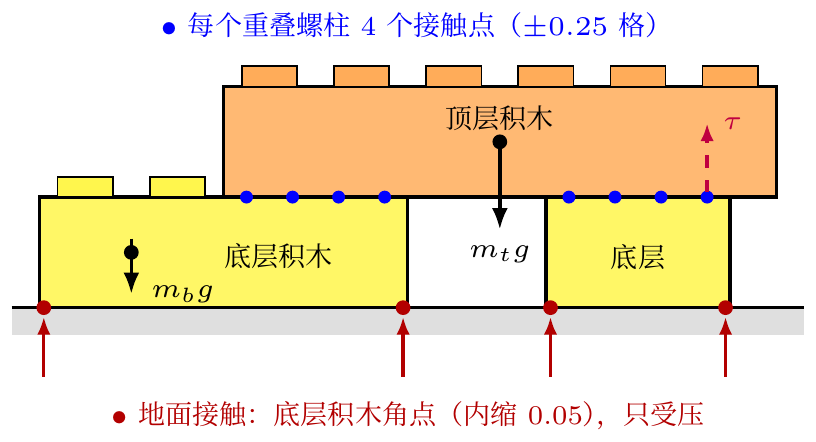
\includegraphics[width=0.95\columnwidth]{figures/image13.png}
\caption{Historical contact-based gravity screening model (source labels in Chinese are retained).}
\end{figure}

\begin{figure}[t]
\centering
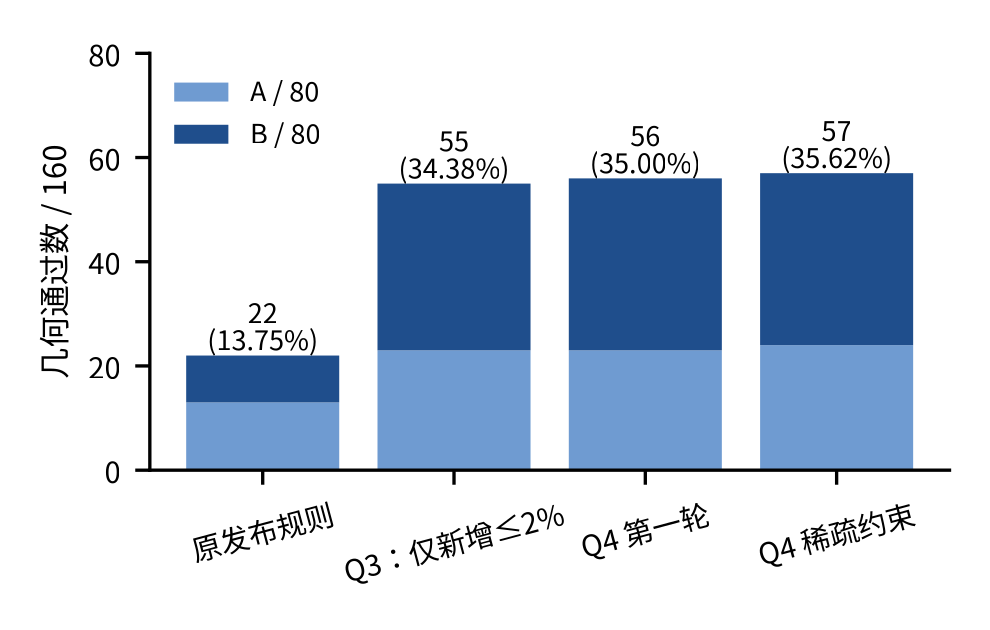
\includegraphics[width=0.95\columnwidth]{figures/image16.png}
\caption{Historical results on a uniform 160-model sample. Version and numerical labels require verification.}
\end{figure}

\begin{figure*}[!htbp]
\centering
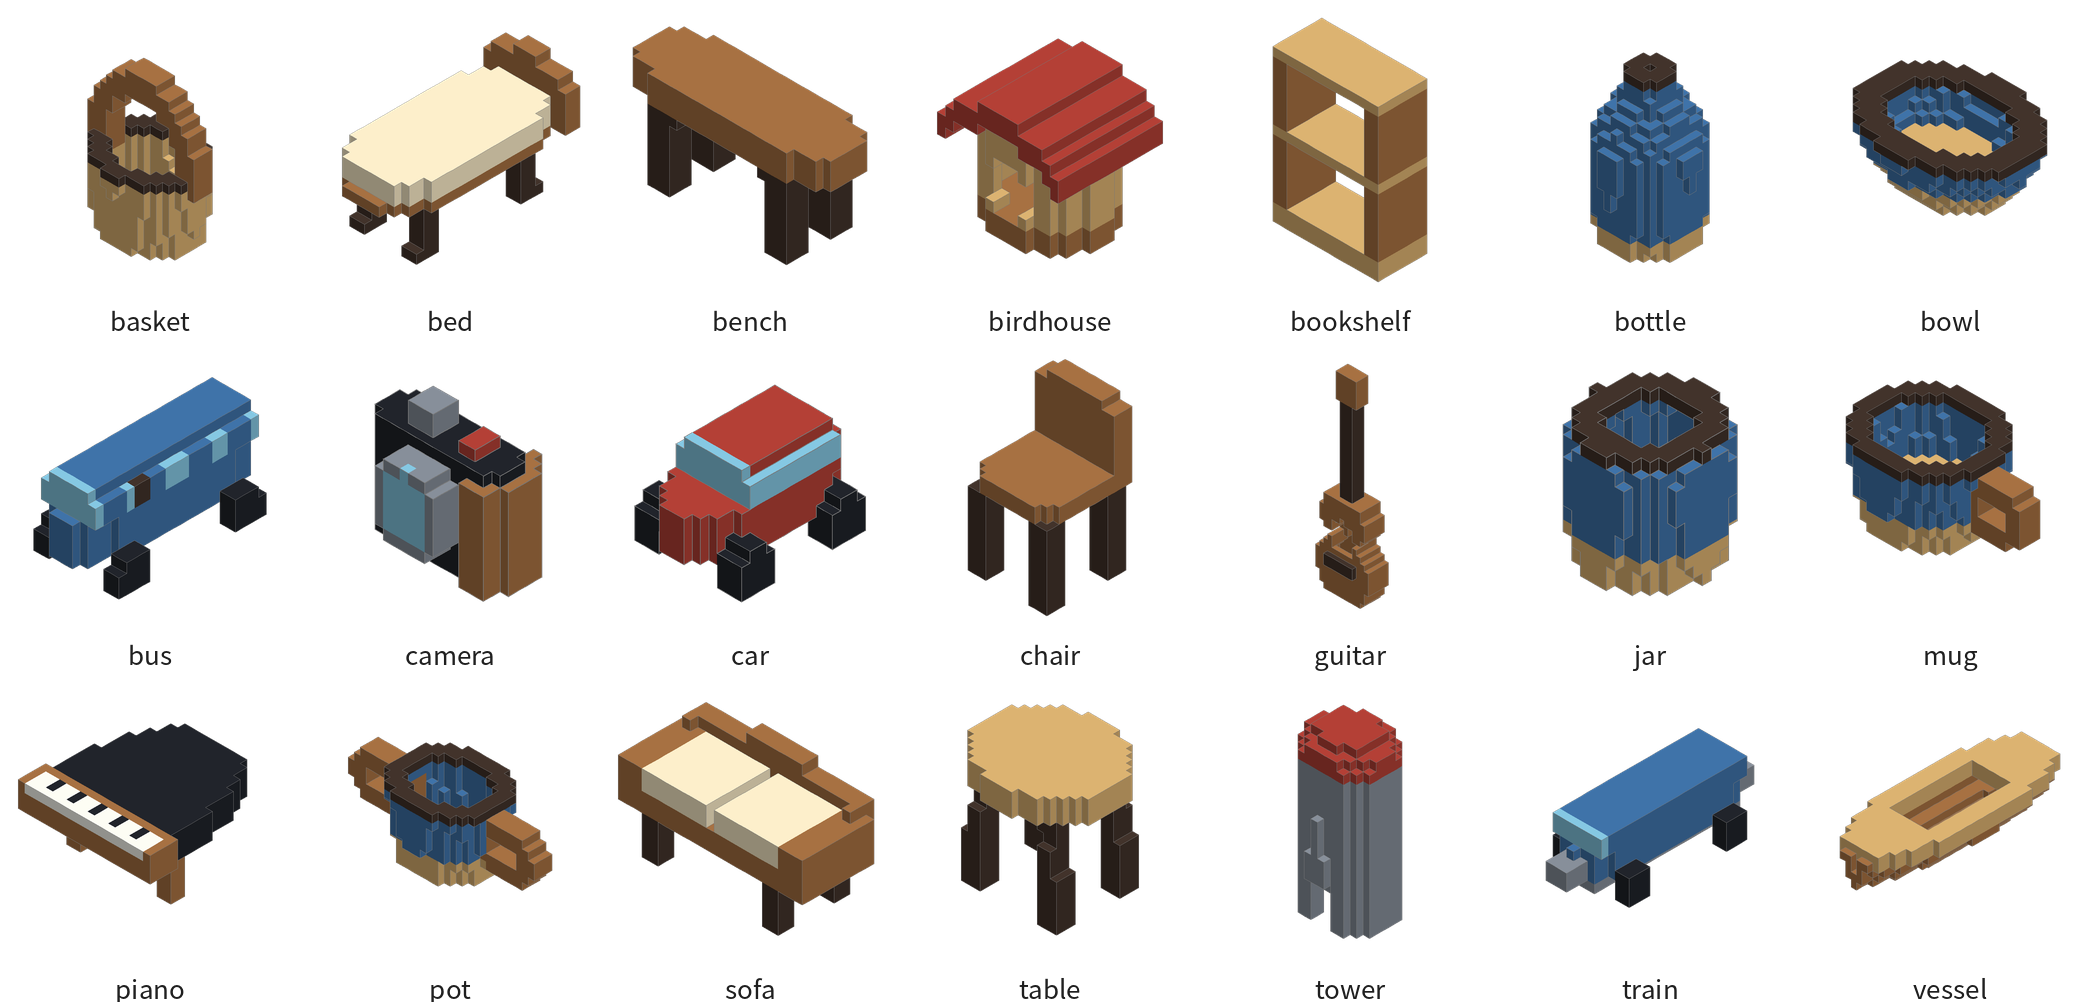
\includegraphics[width=0.475\textwidth]{figures/image7.png}\hfill
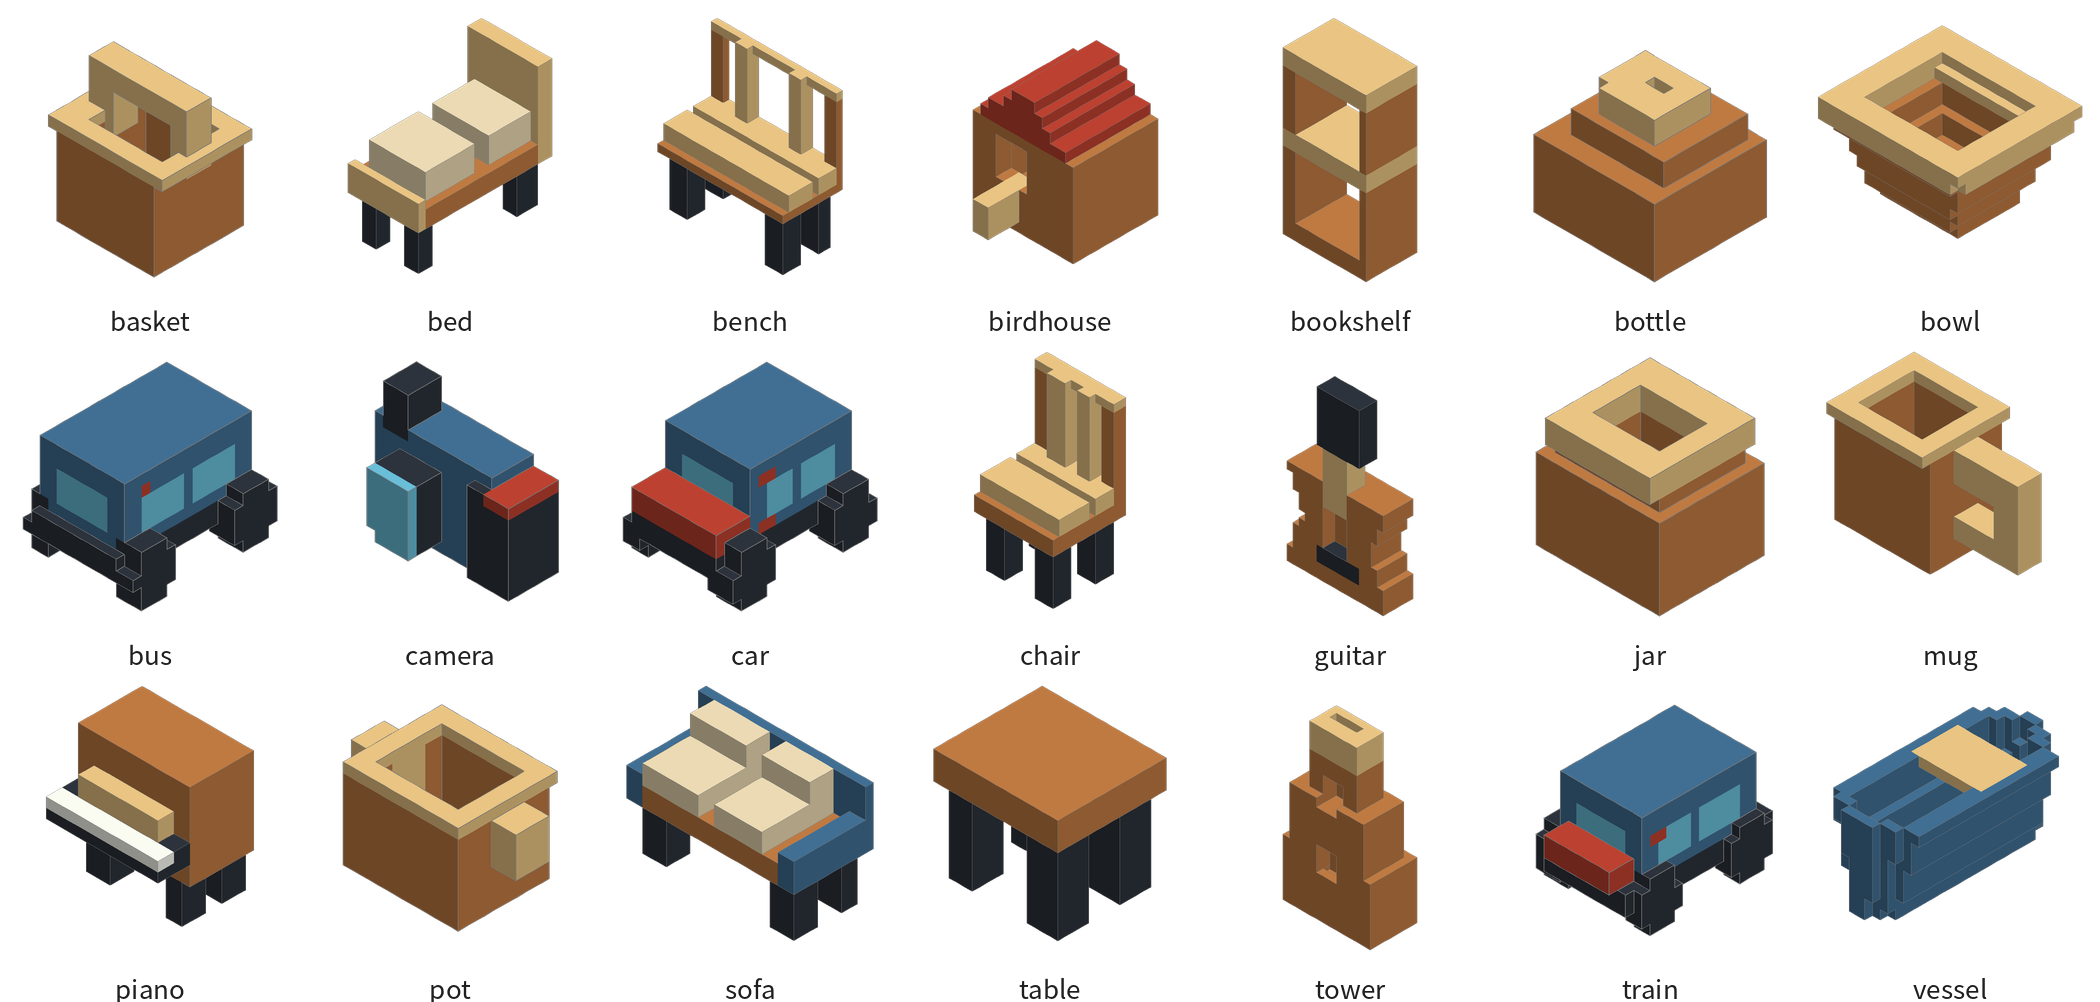
\includegraphics[width=0.475\textwidth]{figures/image8.png}
\caption{Voxel model samples spanning the 21 object categories.}
\end{figure*}

\begin{figure*}[!htbp]
\centering
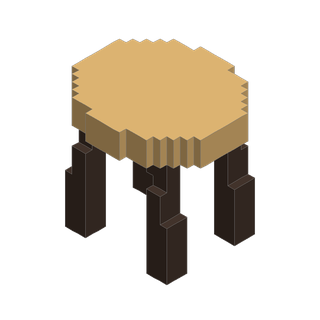
\includegraphics[width=0.118\textwidth]{figures/image4.png}\hfill
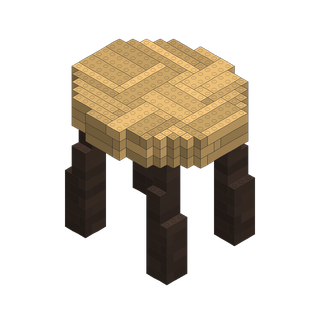
\includegraphics[width=0.118\textwidth]{figures/image5.png}\hfill
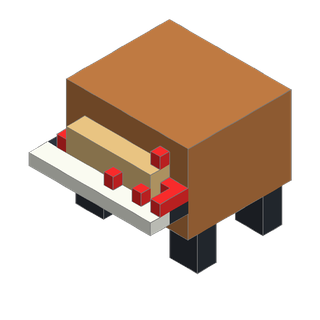
\includegraphics[width=0.118\textwidth]{figures/image2.png}\hfill
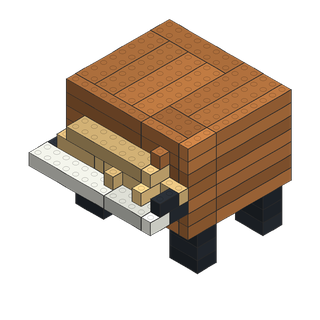
\includegraphics[width=0.118\textwidth]{figures/image3.png}\hfill
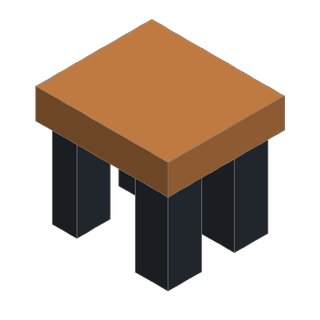
\includegraphics[width=0.118\textwidth]{figures/image9.png}\hfill
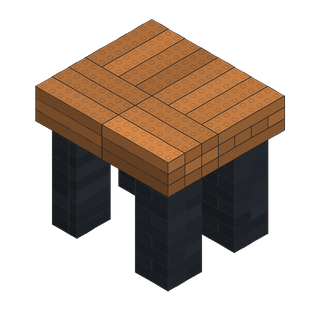
\includegraphics[width=0.118\textwidth]{figures/image10.png}\hfill

\includegraphics[width=0.118\textwidth]{figures/image11.png}\hfill
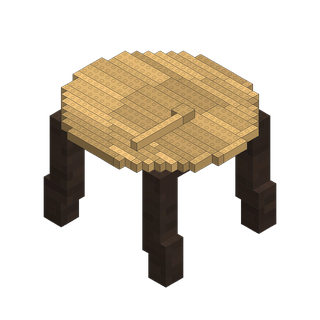
\includegraphics[width=0.118\textwidth]{figures/image12.png}
\caption{Historical examples of voxel targets and brick layouts after local repair.}
\end{figure*}

\begin{figure*}[!htbp]
\centering
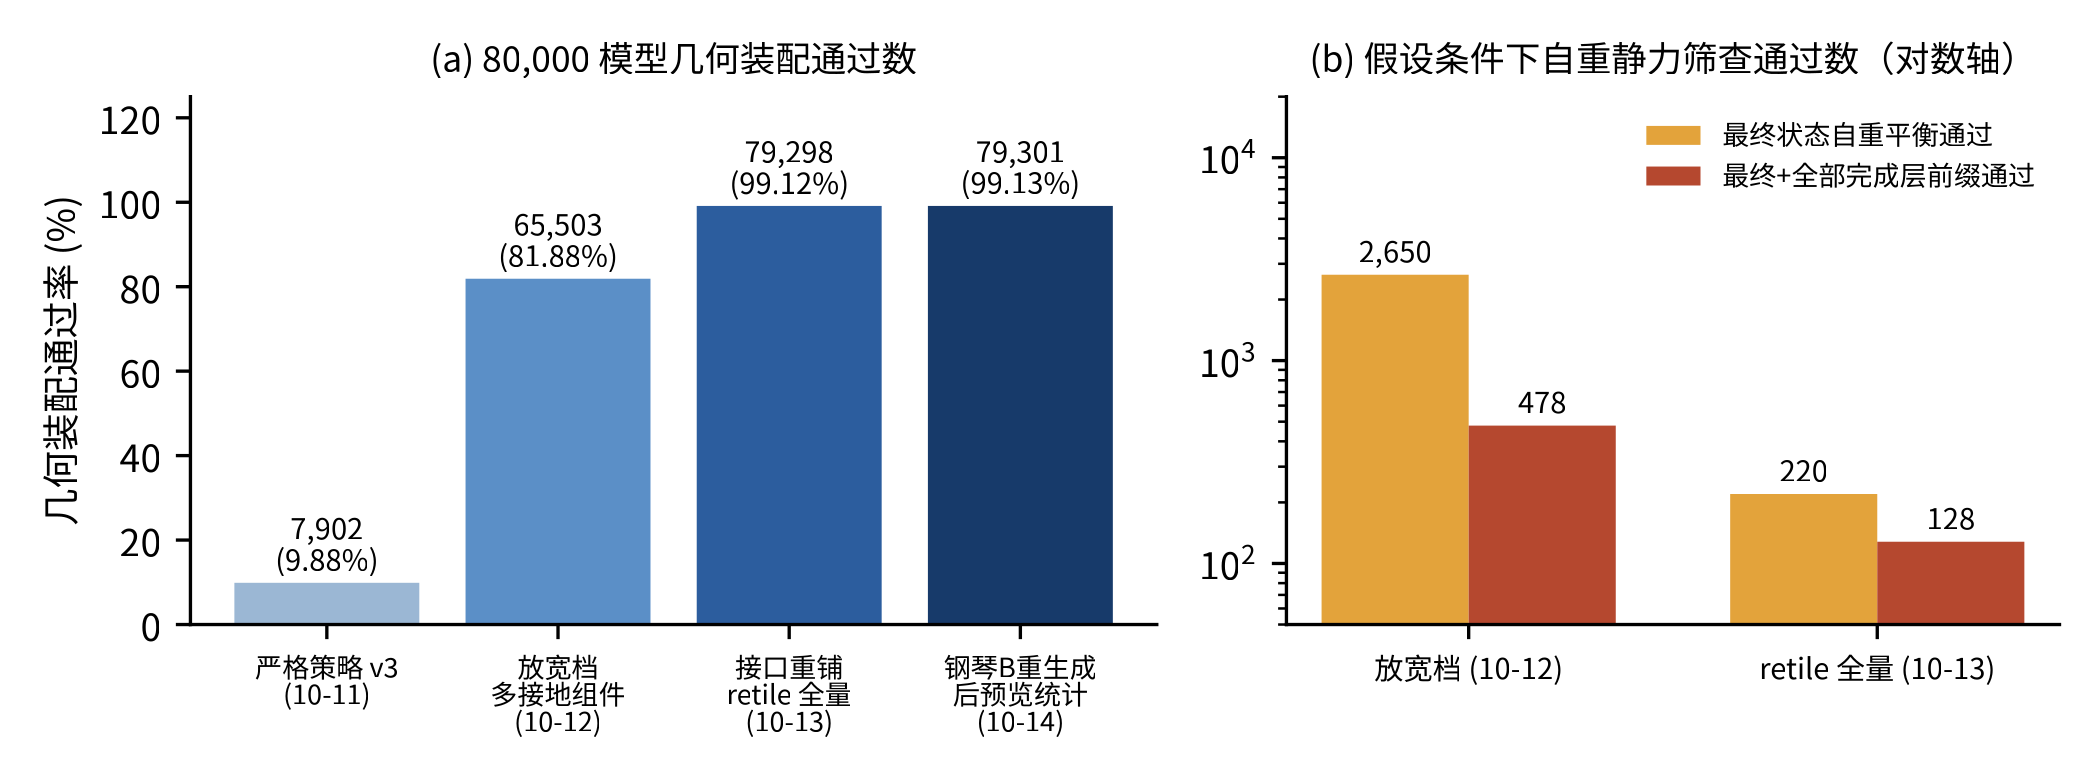
\includegraphics[width=0.70\textwidth]{figures/image14.png}
\caption{Historical comparison of geometric conversion and screening outcomes across releases. Version and numerical labels require verification.}
\end{figure*}

\begin{figure*}[!htbp]
\centering
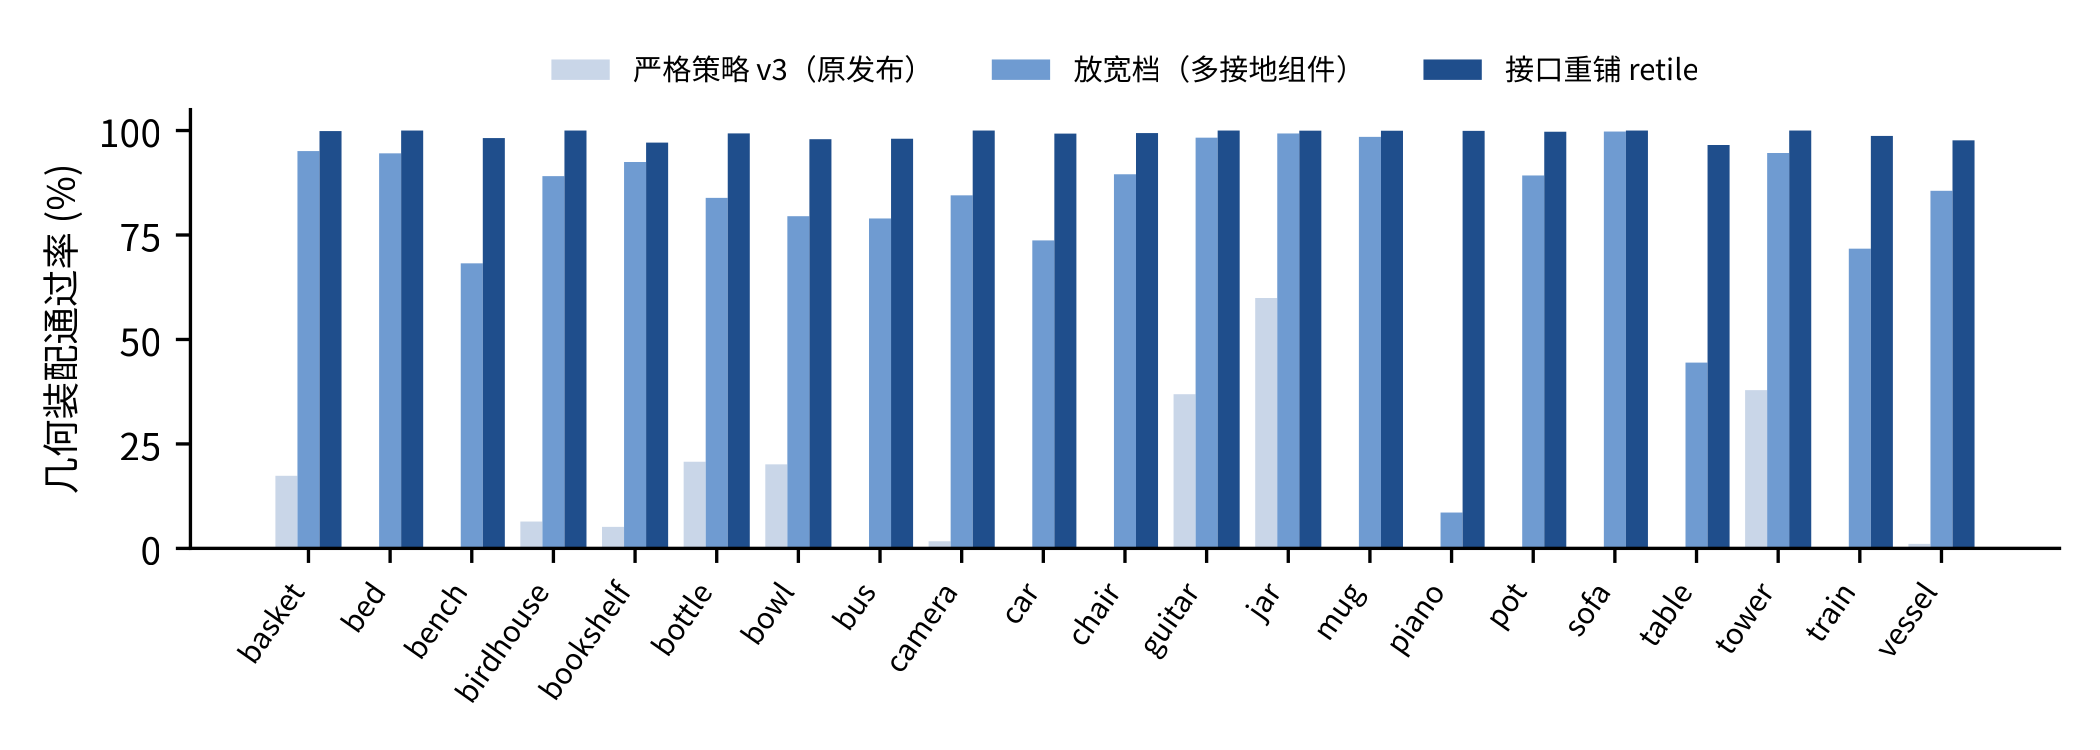
\includegraphics[width=0.70\textwidth]{figures/image15.png}
\caption{Historical category-level geometric pass rates. Version and numerical labels require verification.}
\end{figure*}


\begin{figure*}[!htbp]
\centering
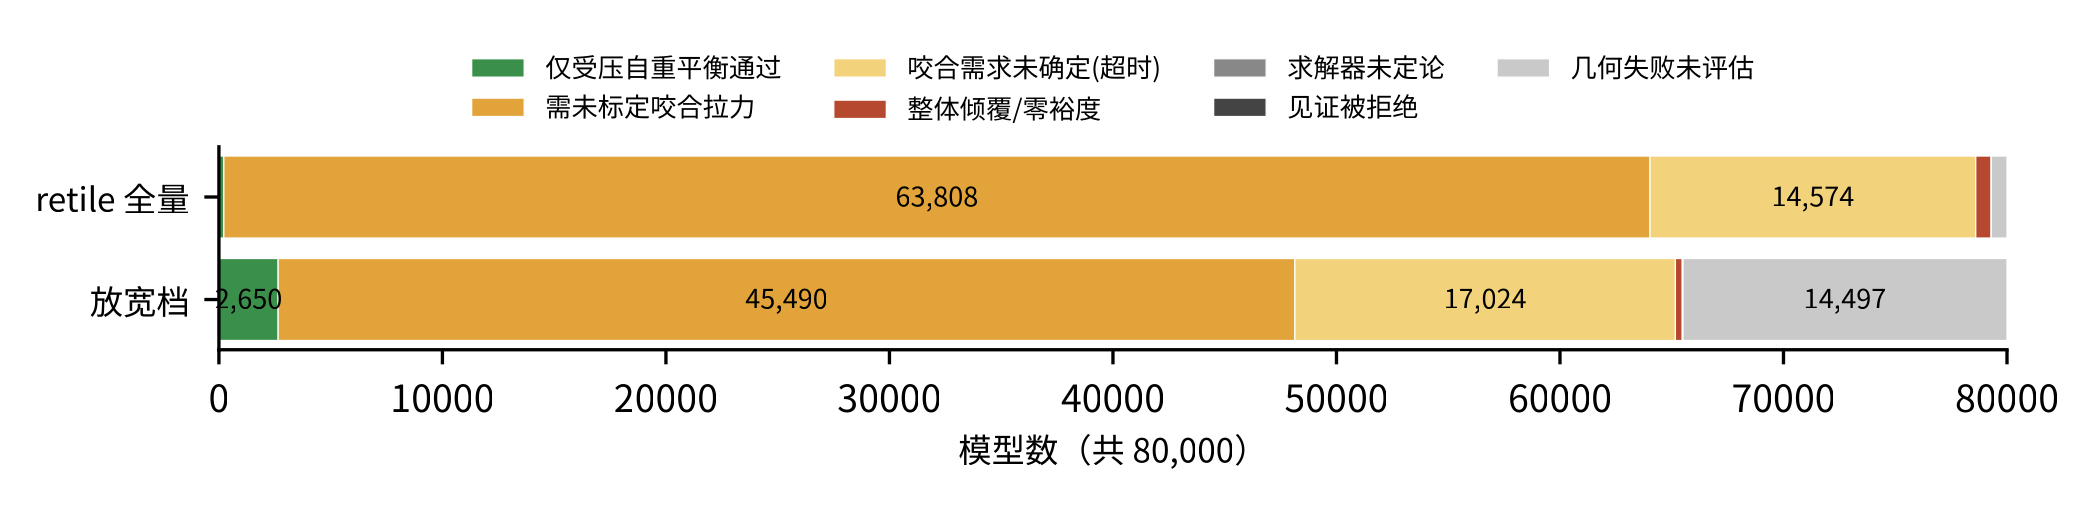
\includegraphics[width=0.70\textwidth]{figures/image17.png}
\caption{Historical distributions of physical screening statuses. Counts refer to the specific releases shown and are kept separate from geometric pass rates.}
\end{figure*}

\FloatBarrier
\section{Technical Appendix: Training Details}
\label{app:training}
Aggregate throughput is 24,448 tokens/s over eight GPUs, and the mean training loss is 0.0273. Evaluation and checkpointing run every 500 steps. With TRL~0.15, the unpacked multi-GPU path hangs after the first backward pass, which is why the TRL~0.17 stack is pinned. Because validation loss is lowest during epoch 2, two epochs would be a more economical setting for future runs (about one third less compute). The full software stack is transformers 4.51.3, trl 0.17.0, peft 0.15.2, datasets 3.6.0, and accelerate 1.6.0, with bf16 precision, gradient checkpointing, and unpacked sequences.

\begin{table}[t]
\centering
\small
\begin{tabular}{lrr}
\toprule
Progress & Step & Validation loss \\
\midrule
Start & 500 & 0.1410 \\
--- & 1,500 & 0.0950 \\
--- & 10,500 & 0.0509 \\
--- & 22,500 & 0.0404 \\
$\approx$ End of epoch 1 & 44,500 & 0.0337 \\
--- & 65,500 & 0.0316 \\
Best (epoch 1.77) & 79,000 & 0.0308 \\
End of epoch 3 & 133,860 & 0.0339 \\
\bottomrule
\end{tabular}
\caption{Validation loss on the 2,000-sample validation subset. One epoch is $\approx$44,620 steps; the nearest evaluation to the end of epoch 1 is step 44,500.}
\label{tab:eval-loss}
\end{table}

% BrickGPT-paper column verified against arXiv:2505.05469 (Sec. 5.1 and Appendix A training details).
\begin{table}[t]
\centering
\scriptsize
\setlength{\tabcolsep}{3pt}
\begin{tabular}{@{}l>{\raggedright\arraybackslash}p{0.31\columnwidth}>{\raggedright\arraybackslash}p{0.34\columnwidth}@{}}
\toprule
Dimension & BrickGPT paper & Official Qwen3 script (ours) \\
\midrule
Base model & LLaMA-3.2-1B-Instruct & Qwen3-1.7B \\
LoRA & $r=32$, $\alpha=16$, dropout $0.05$, $q$/$v$ only (3.4M params) & $r=16$, $\alpha=32$, all linear layers \\
Learning rate & $2{\times}10^{-3}$ (AdamW) & $10^{-4}$ \\
Effective batch & 64 & 8 \\
Max length & 4,096 & 8,192 \\
Epochs & 3 & 3 \\
Hardware & 8$\times$RTX A6000, 12\,h & 8$\times$4090D, 25.3\,h \\
Data & StableText2Brick, 47k structures / 240k prompts & BrickMore-48, 79.3k models / 396,610 samples \\
\bottomrule
\end{tabular}
\caption{Our configuration versus the original BrickGPT paper \cite{brickgpt}. BrickGPT-paper values are taken from Sec.~5.1 and Appendix~A of arXiv:2505.05469 (base model, LoRA $r{=}32$, $\alpha{=}16$, dropout $0.05$, $q$/$v$ only with 3.4M parameters, AdamW learning rate $0.002$, global batch 64, 4096-token length filter, 3 epochs, 8$\times$RTX A6000 and 12\,h, and 47k+ structures / 240k prompts). The data organization, instruction template, absence of thinking mode, and LoRA paradigm follow BrickGPT; concrete hyperparameters follow the official Qwen3 adaptation, with the budget adjusted for the larger world, library, and corpus.}
\label{tab:brickgpt-recipe}
\end{table}

\FloatBarrier
\section{Technical Appendix: Additional Evaluation Material}
\label{app:eval}
This appendix retains the qualitative gallery and historical baseline-comparison figures from the supplied reference material.

\begin{figure*}[t]
\centering
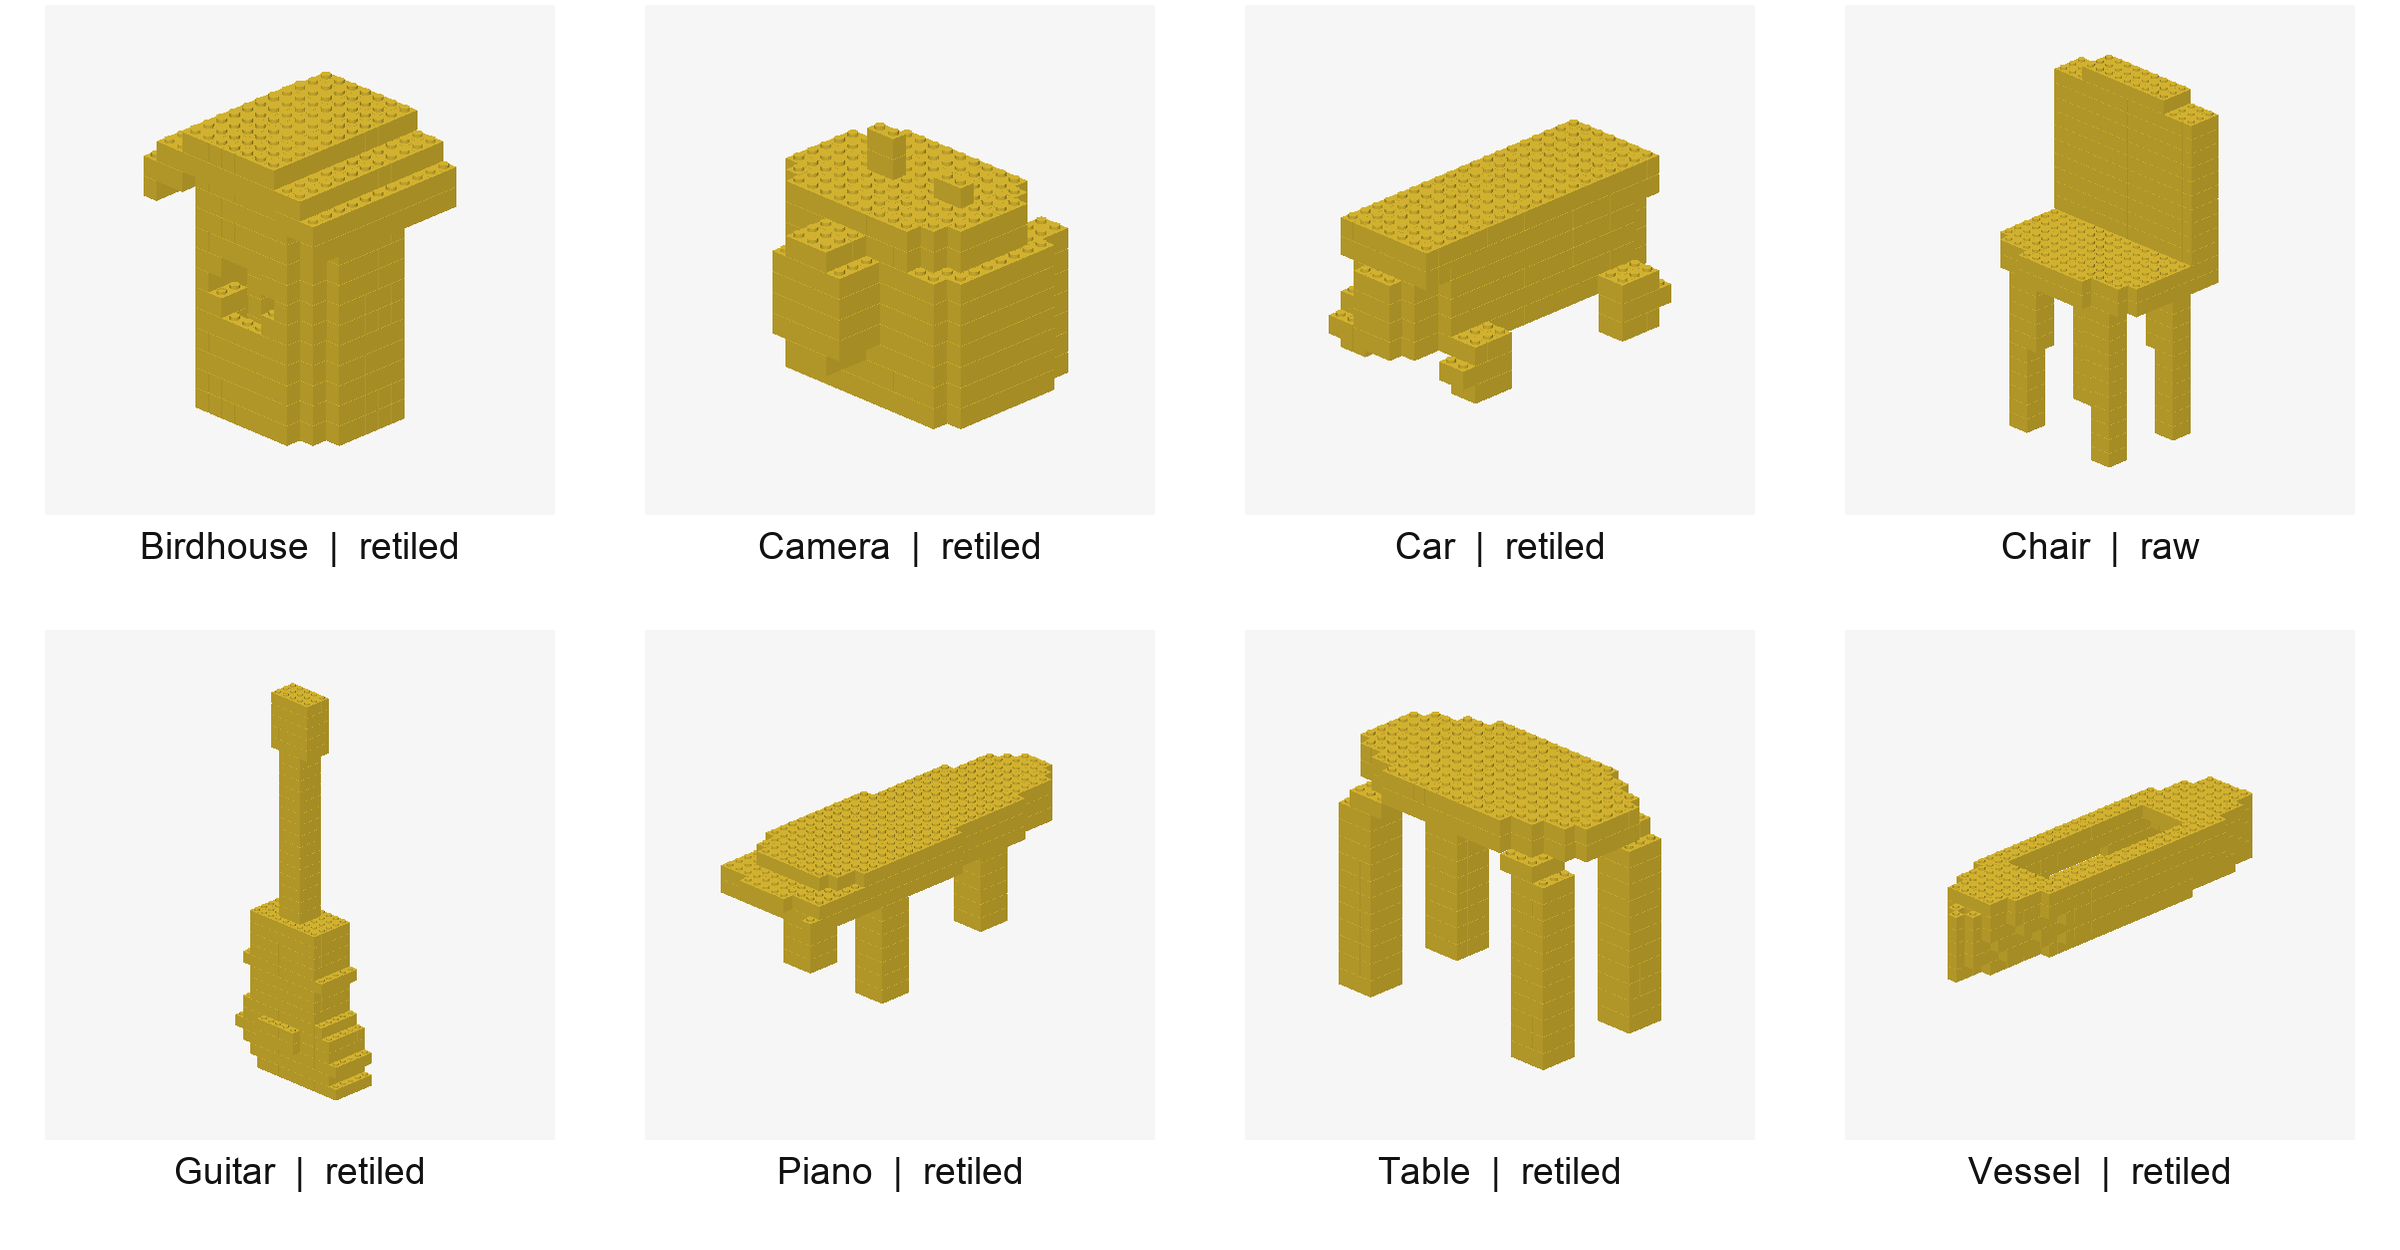
\includegraphics[width=0.75\textwidth]{figures/generated_gallery.png}
\caption{Selected BrickForma outputs from the 114-prompt evaluation, rendered with the uniform evaluation protocol (not photographs of physical assemblies). In this gallery, one chair is raw and the other outputs are retiled; in the full main comparison, 4 of the 114 BrickForma outputs are raw.}
\label{fig:gallery}
\end{figure*}

\begin{figure*}[!htbp]
\centering
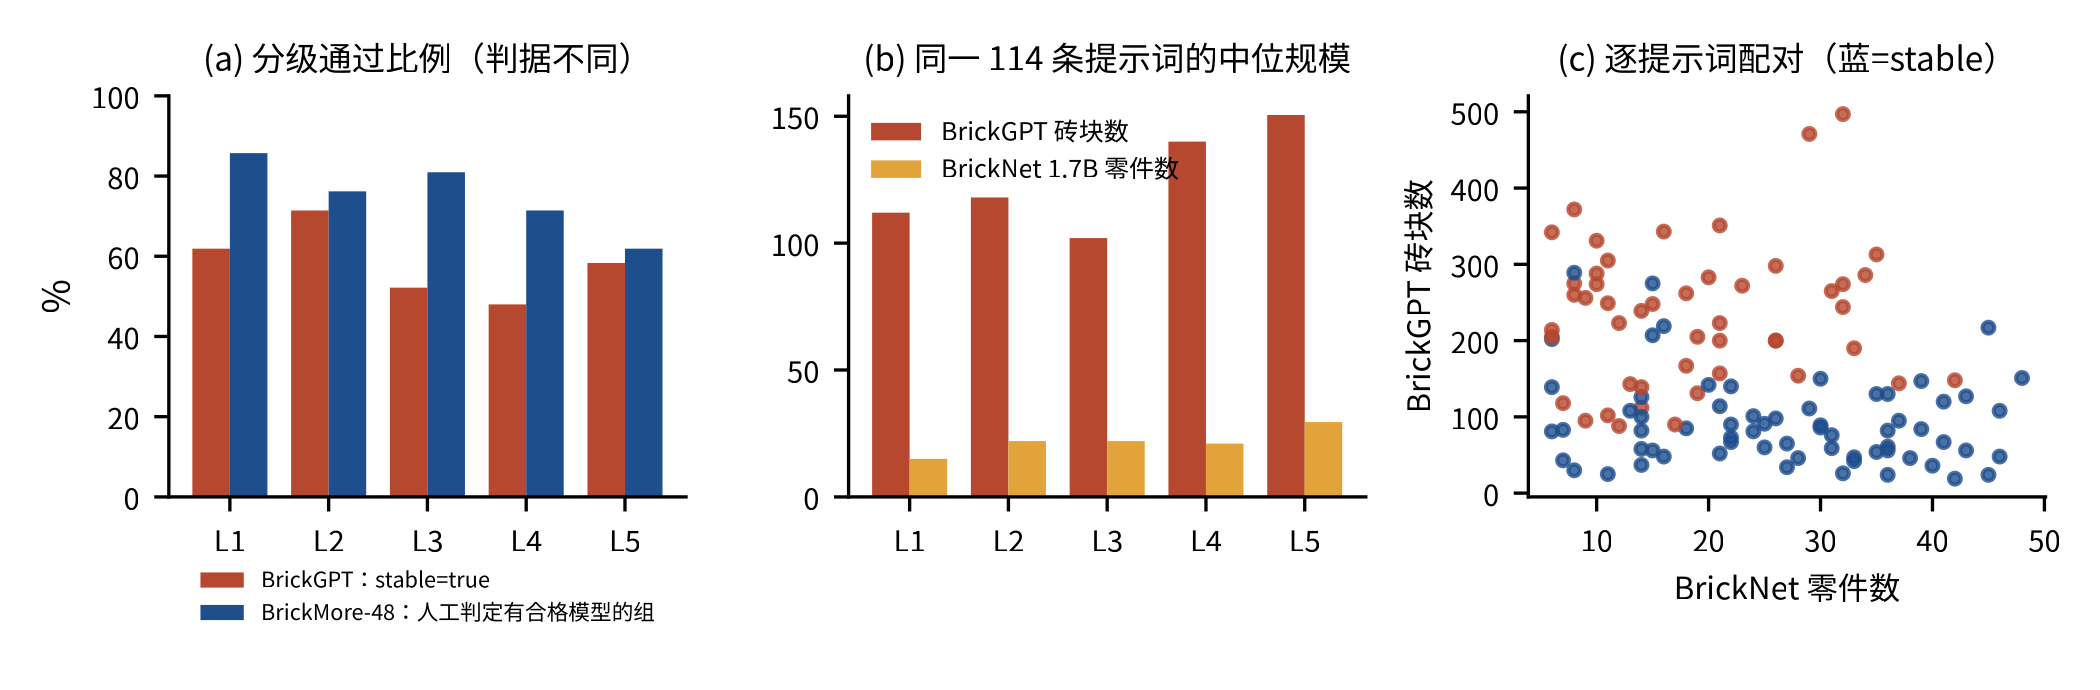
\includegraphics[width=0.70\textwidth]{figures/image18.png}
\caption{Historical baseline comparison with differing acceptance criteria; not the current matched main comparison.}
\end{figure*}

\begin{figure*}[!htbp]
\centering
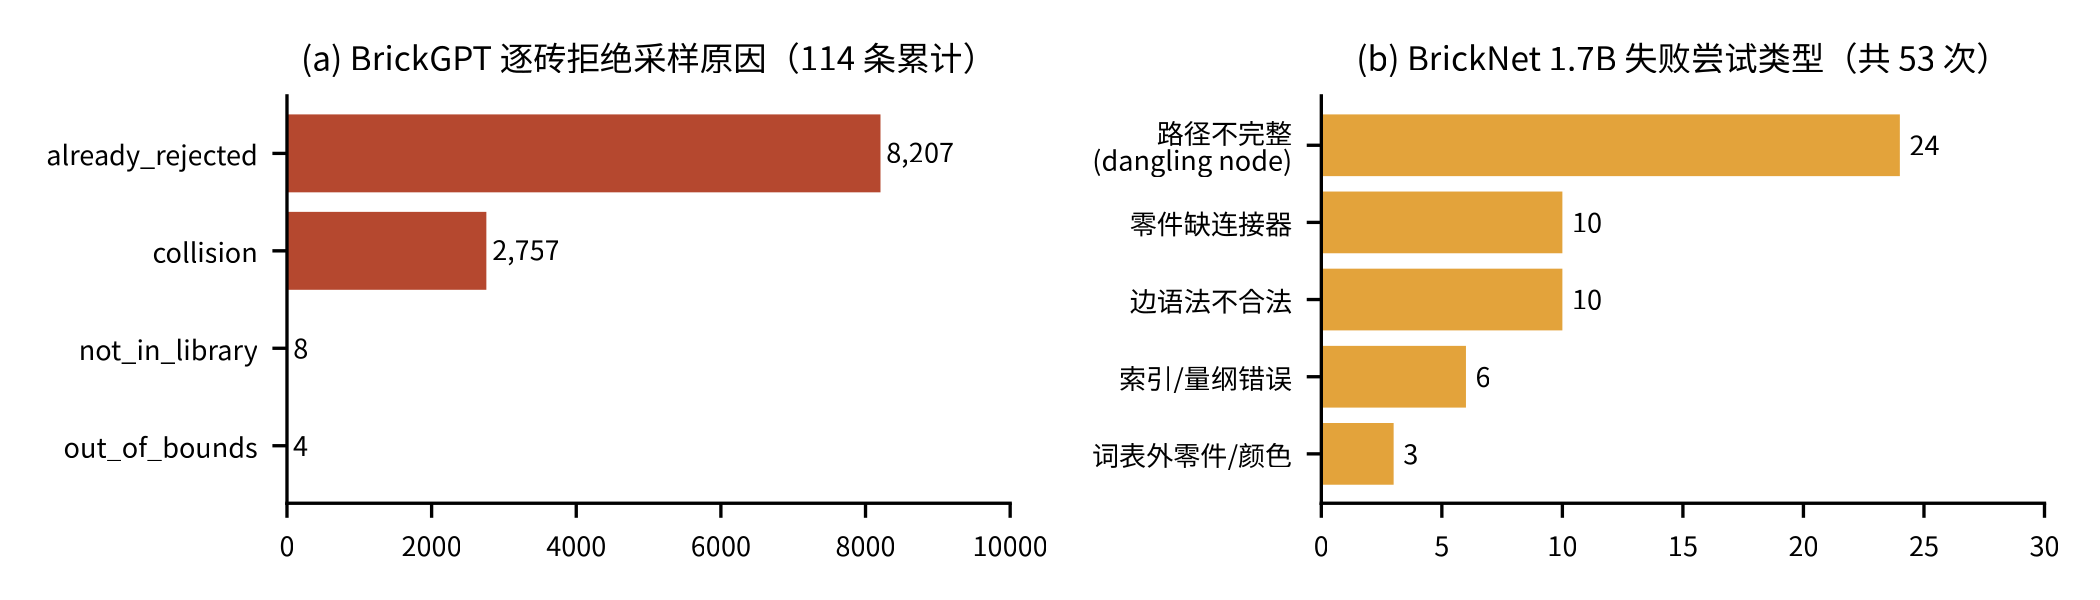
\includegraphics[width=0.70\textwidth]{figures/image19.png}
\caption{Historical failure categories in the supplied reference; sample definitions require verification.}
\end{figure*}

\begin{figure*}[t]
\centering
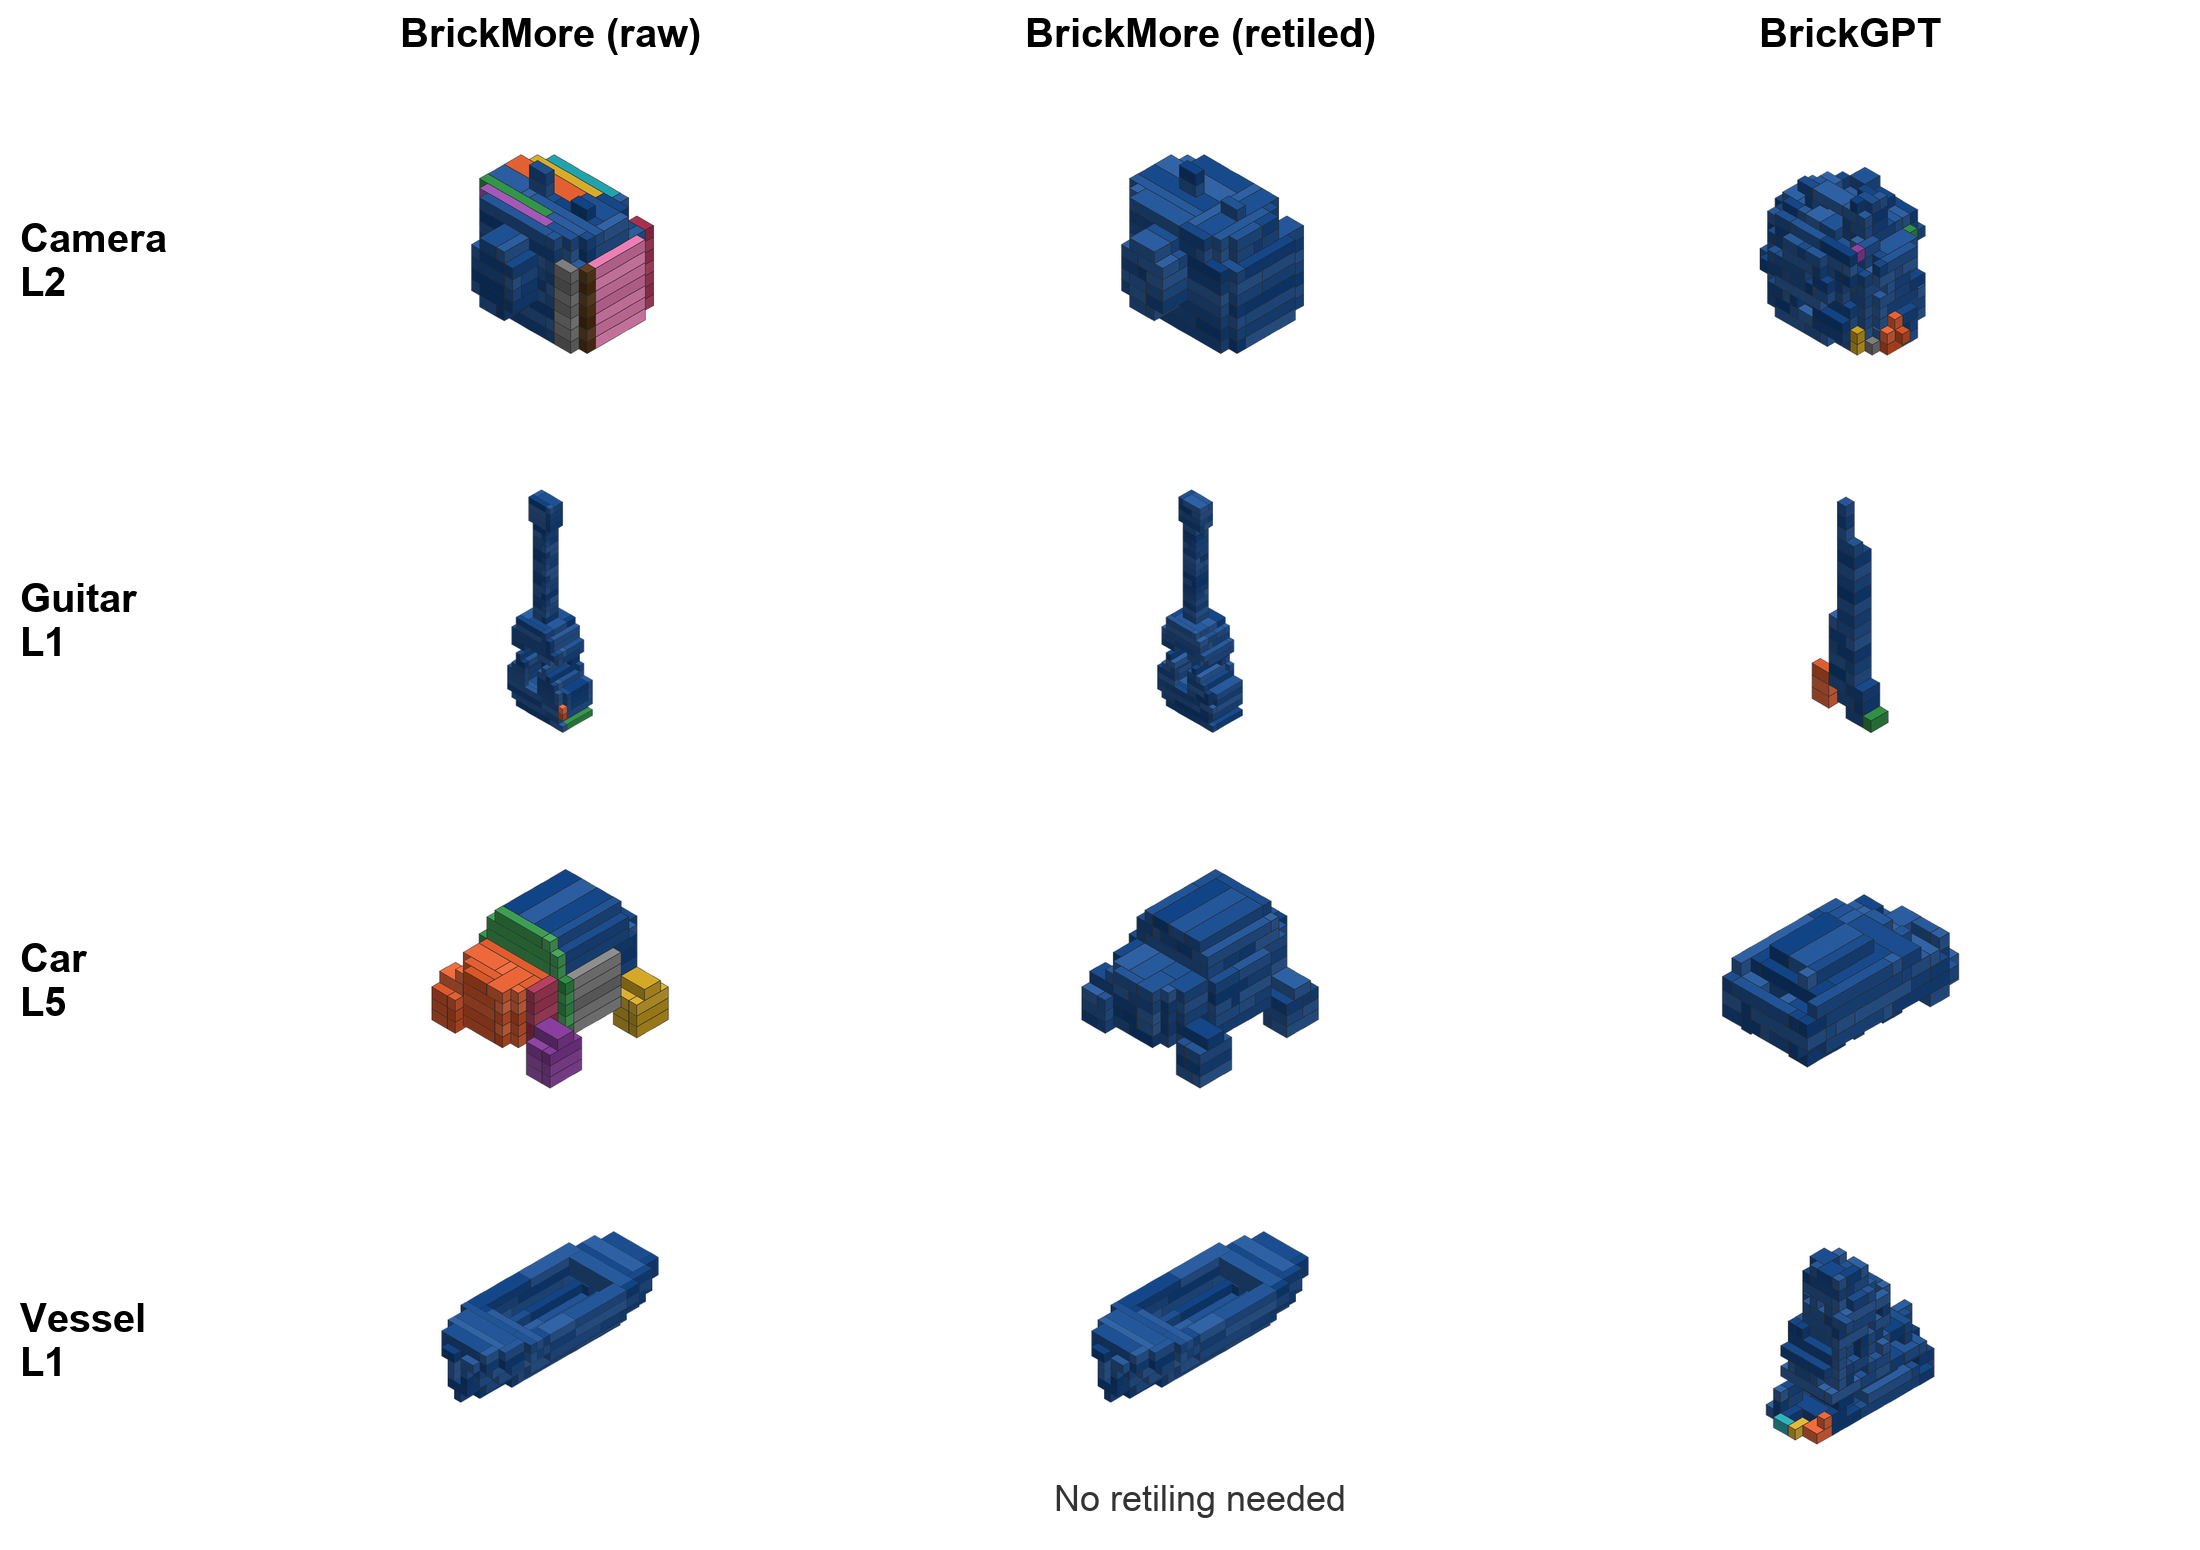
\includegraphics[width=0.54\textwidth]{figures/original_comparison.png}
\caption{Qualitative historical examples from the supplied reference. Column labels distinguish raw BrickMore, retiled BrickMore, and BrickGPT outputs.}
\end{figure*}

\section{Technical Appendix: Historical Tables}
\label{app:historical}
The following transcribed tables preserve the historical reference material. They use different versions or evaluation criteria and are not substitutes for the current main comparison. Dashes indicate missing entries in the supplied source.
\begin{table*}[t]
\centering\scriptsize
\begin{minipage}[t]{0.48\textwidth}
\centering
\begin{tabular}{lr}\toprule
Item & Historical value \\ \midrule
Voxel models & 80,000 (40,000 per batch) \\
Categories / structural families & 21 / 40 per category \\
Grid / voxel count & $48^3$ / 750--1,250 \\
Prompt records & 400,000 (five bilingual records per model) \\
Uniqueness & 80,000 unique; 0 A/B duplicates \\
Overlap with historical hashes & 0 / 55,255 \\
Retile geometry passes & 79,298 (99.12\%) \\
Bricks in full preview & 12,718,389 \\
Final gravity equilibrium passes & 220 \\
Final and layer-prefix passes & 128 \\
\bottomrule\end{tabular}
\caption{Historical dataset statistics transcribed from the supplied reference. The geometry count refers to the old retile release, not the later integrated count. Verify the preview and physical-screening totals against version-matched reports.}
\end{minipage}\hfill
\begin{minipage}[t]{0.48\textwidth}
\centering
\setlength{\tabcolsep}{4pt}
\begin{tabular}{lrrr}\toprule
Item & BrickGPT & BrickNet 1.7B & BrickMore-48 \\ \midrule
Representation & $20^3$ bricks & Assembly graph & $48^3$ bricks \\
Criterion & stable & Parseable & -- \\
Passes & 66/114 & 114/114 & -- \\
Median parts & 126.5 & 22 & -- \\
Range & 19--497 & 6--48 & -- \\
Mean time (s) & 189.6 & -- & -- \\
\bottomrule\end{tabular}
\caption{Historical baseline table in the source reference. These criteria differ, and missing BrickMore entries were marked TODO. This is not the current matched four-metric main table.}
\end{minipage}
\end{table*}

\begin{table*}[t]\centering\scriptsize
\begin{tabular}{llrrrrr}\toprule
Version & Connectivity & Voxel changes & Passes & Rate & Final & Final + prefixes \\ \midrule
Strict v3 & Single; support $\geq$10\%, overhang $\leq$2 & None & 7,902 & 9.88\% & -- & -- \\
Relaxed & Each component grounded & +428,278 / -38,230 & 65,503 & 81.88\% & 2,650 & 478 \\
Retile & Each component grounded & +228,582 / -125 & 79,298 & 99.12\% & 220 & 128 \\
\midrule
\multicolumn{7}{l}{Uniform 160-model sample (seed 38177); not full-dataset results} \\
Baseline & Single stud-connected component & None & 22 & 13.75\% & -- & -- \\
Q3 & Single stud-connected component & Added $\leq$2\% & 55 & 34.38\% & 8 & 2 \\
Q4 (sparse) & Single stud-connected component & Added + removed $\leq$2\% & 57 & 35.63\% & 8 & 2 \\
\bottomrule\end{tabular}
\caption{Historical conversion-strategy table from the reference. Full-dataset and 160-model sample rows use different scopes; connectivity rules also differ. Final and prefix columns report screening outcomes under the stated historical assumptions.}
\end{table*}

\begin{table*}[t]\centering\scriptsize
\begin{tabular}{lrrrrl}\toprule
Level & $n$ & BrickGPT stable & BrickGPT median bricks & BrickNet median parts & BrickMore-48 \\ \midrule
L1 & 21 & 13 & 112 & 15 & -- \\
L2 & 21 & 15 & 118 & 22 & -- \\
L3 & 23 & 12 & 102 & 22 & -- \\
L4 & 25 & 12 & 140 & 21 & -- \\
L5 & 24 & 14 & 150.5 & 29.5 & -- \\
\bottomrule\end{tabular}
\caption{Historical level-wise baseline table transcribed from the reference. The original BrickMore column was incomplete, and the other columns use different criteria.}
\end{table*}

\begin{table*}[t]\centering\scriptsize
\begin{tabular}{lrrrr}\toprule
Method and source & $P_{\mathrm{inv}}$ & VQA & PE & SigLIP2 \\ \midrule
BrickGPT (literature, as transcribed) & 0.063 & 0.050 & 0.157 & 0.052 \\
BrickNet 1.7B (literature, as transcribed) & 0.260 & 0.593 & 0.282 & 0.631 \\
BrickGPT (114 prompts, historical placeholder) & -- & -- & -- & -- \\
BrickNet (114 prompts, historical placeholder) & -- & -- & -- & -- \\
BrickMore-48 (114 prompts, historical placeholder) & -- & -- & -- & -- \\
\bottomrule\end{tabular}
\caption{Original reference table with literature values and historical placeholders. Literature values use another evaluation set and must not be directly compared with the present 114-prompt results; the precise $P_{\mathrm{inv}}$ definition and direction require checking against the original publication.}
\end{table*}

\FloatBarrier
\end{document}
